% !TEX program = xelatex
%==============================================================================
%  Representation as a Computational Resource in Quantum Compilation
%  Group seminar / AQIS 2026 poster-session rehearsal
%
%  Built from AQIS26_Poster/BEAMER_SPEC.md.
%  Section order is Part I -> Part VI  ==  spec  §0 -> §1 -> §2 -> §3 -> §4 -> §5.
%  Part VII (appendix) follows §5 and is backup only.
%
%  Compile:  xelatex main.tex   (twice, for \tableofcontents)
%==============================================================================
\documentclass[aspectratio=169,10pt]{beamer}

% ---- Theme: classic blue (Warsaw headline + Madrid-style infolines footer) --
\usetheme{Warsaw}              % fallback: \usetheme{default} + \usecolortheme{whale}
% There are no subsections, so give the section navigation the full bar width.
% (Warsaw's default split headline gives sections only half the width, which
%  wraps at 5+ sections and then under-reserves the page height by 1.4pt.)
\useoutertheme[subsection=false]{smoothbars}
\setbeamercovered{invisible}

% Madrid's three-part footline: author (institute) | title | date / page.
\setbeamertemplate{footline}{%
  \leavevmode%
  \hbox{%
  \begin{beamercolorbox}[wd=.30\paperwidth,ht=2.25ex,dp=1ex,center]%
                       {author in head/foot}%
    \usebeamerfont{author in head/foot}\footcellauthor
  \end{beamercolorbox}%
  \begin{beamercolorbox}[wd=.46\paperwidth,ht=2.25ex,dp=1ex,center]%
                       {title in head/foot}%
    \usebeamerfont{title in head/foot}\insertshorttitle
  \end{beamercolorbox}%
  \begin{beamercolorbox}[wd=.24\paperwidth,ht=2.25ex,dp=1ex,right]%
                       {date in head/foot}%
    \usebeamerfont{date in head/foot}\insertshortdate{}\hspace*{2em}%
    \insertframenumber{}\,/\,\inserttotalframenumber\hspace*{2ex}
  \end{beamercolorbox}}%
  \vskip0pt%
}
% swapped for a BACKUP marker once \appendix starts
\newcommand{\footcellauthor}{\insertshortauthor~~(\insertshortinstitute)}

% Inline \frac / tall subscripts sit inside \footnotesize lists in several
% frames. Raise the minimum interline gap so TeX separates any over-tall line
% automatically, instead of letting a numerator ride into the line above.
\setlength{\lineskiplimit}{2.2pt}
\setlength{\lineskip}{2.2pt}

% reclaim the vertical space the headline and footline cost
\setbeamersize{text margin left=5mm,text margin right=5mm}
\setbeamerfont{frametitle}{size=\normalsize,series=\bfseries}
\setbeamerfont{block title}{size=\small}
\addtobeamertemplate{block begin}{\vspace{-0.6mm}}{\vspace{-0.6mm}}
\addtobeamertemplate{block end}{}{\vspace{-1.2mm}}

\usepackage{amsmath,amsthm,mathtools}   % amssymb dropped: unicode-math supplies
\usepackage{tikz}                       % \blacksquare, \blacktriangleright, \mathbb
\usetikzlibrary{arrows.meta,positioning,calc,decorations.pathreplacing,patterns}
\usepackage{booktabs}
\usepackage{array}
\usepackage{pifont}
\usepackage{relsize}
\usepackage{xcolor}
\setbeamertemplate{navigation symbols}{}
\setbeamertemplate{caption}[numbered]

%---- Fonts -------------------------------------------------------------------
% Latin text: Anthropic Serif Web. The family ships Regular + Italic only, so
% every bold weight in the deck (frame titles, block titles, \hd, \textbf) is
% synthesised by XeTeX via AutoFakeBold.
\usefonttheme{serif}
\usepackage{fontspec}
\setmainfont{Anthropic Serif Web}[AutoFakeBold=1.9]
\setsansfont{Anthropic Serif Web}[AutoFakeBold=1.9]  % beamer asks for sans a lot

% Math: TeX Gyre Pagella Math (Palatino-style serif math).
\usepackage{unicode-math}
\setmathfont{texgyrepagella-math.otf}

% CJK: Songti SC, with the bold weight faked as well (Songti has no true bold).
\usepackage[UTF8,scheme=plain,fontset=none]{ctex}
\setCJKmainfont{Songti SC}[AutoFakeBold=2.2]
\setCJKsansfont{Songti SC}[AutoFakeBold=2.2]
\setCJKmonofont{Songti SC}

% Uncomment ONE of the following to render the Chinese speaker notes:
% \setbeameroption{show notes}
% \setbeameroption{show notes on second screen=right}

% ---- Language switch (§0.2) ------------------------------------------------
% \zhtrue  ==> frame/section titles switch to Chinese.
\newif\ifzh \zhfalse
\newcommand{\bl}[2]{\ifzh #2\else #1\fi}

% ---- Theorem environments (§0.3) -------------------------------------------
\newtheorem{claim}{Claim}
\newtheorem{lemma2}{Lemma}
\newtheorem{prop2}{Proposition}
\theoremstyle{definition}
\newtheorem{defn}{Definition}
\newtheorem{remark2}{Remark}

% lightweight proof block (keeps full control inside frames)
\newenvironment{prf}[1][Proof]%
  {\par\smallskip\noindent\textit{#1.}\ \ignorespaces}%
  {\hfill$\blacksquare$\par\smallskip}

% ---- Notation macros (§0.3) ------------------------------------------------
\newcommand{\dproj}{d_{\mathrm{proj}}}
\newcommand{\op}{\mathrm{op}}
\newcommand{\Fb}{\mathbb{F}_2}
\newcommand{\ZQ}{\mathbb{Z}_Q}
\newcommand{\cd}[1]{\langle\!\langle #1 \rangle\!\rangle}
\newcommand{\Bcut}{B_{\mathrm{cut}}}
\newcommand{\Ldelta}{L_\delta(m,K)}
\newcommand{\hbin}{h_2}

% ---- Callout styles (§0.4) -------------------------------------------------
% calblue is the Warsaw structure blue, so the TikZ figures match the theme
\definecolor{calblue}{rgb}{0.2,0.2,0.7}
\definecolor{mustred}{HTML}{A11B1B}
\definecolor{softgrey}{HTML}{EDEDF5}

% "must answer" callout: visually heaviest object in the deck
\newenvironment{mustanswer}[1][Must answer]{%
  \setbeamercolor{block title}{bg=mustred,fg=white}%
  \setbeamercolor{block body}{bg=mustred!8,fg=black}%
  \begin{block}{\raisebox{-0.5pt}{$\blacktriangleright$}\; #1}}%
  {\end{block}}

% ordinary callout
\newenvironment{callout}[1][]{%
  \setbeamercolor{block title}{bg=calblue,fg=white}%
  \setbeamercolor{block body}{bg=calblue!7,fg=black}%
  \begin{block}{#1}}%
  {\end{block}}

\newcommand{\hd}[1]{\textbf{\color{calblue}#1}}

% ---- Bilingual layer -------------------------------------------------------
% Slide bodies stay English (§0.2); a smaller Chinese line is set underneath
% the frame title and underneath each key assertion. Technical nouns are left
% in English on purpose. Both are suppressed when \zhtrue (the body is already
% Chinese then, so the gloss would be a duplicate).
\definecolor{cngloss}{HTML}{3A3A55}
\setbeamerfont{framesubtitle}{size=\scriptsize,series=\mdseries}
\setbeamercolor{framesubtitle}{fg=white}
% Chinese half of a bilingual section title (TOC + bookmarks only)
% Chinese line under the frame title
\newcommand{\zhsub}[1]{\ifzh\else\framesubtitle{#1}\fi}
% Chinese annotation lines inside TikZ nodes. Two rules learned the hard way:
% (a) plain \\ only -- an optional argument like \\[-1mm] is eaten by the
%     TikZ path parser; (b) never name these in the \tikz@ namespace.
\newcommand{\zhtik}[1]{\ifzh\else{\tiny\color{cngloss}#1}\fi}
\newcommand{\zhtikem}[1]{\ifzh\else{\tiny\color{mustred}#1}\fi}
% Chinese line under a key assertion, inside or outside a block
% one step smaller than whatever the surrounding text is, so the gloss stays
% subordinate on \scriptsize frames too
\newcommand{\cn}[1]{\ifzh\else
  \par\vspace{0.35mm}{\normalfont\relsize{-1}\color{cngloss}#1}\par\fi}

% ---- Section outline frames (§0.4) -----------------------------------------
% Hand-written bilingual outline. (\tableofcontents cannot carry the Chinese:
% section titles are moving arguments, and \relsize/\color loop there.)
\newcommand{\olitem}[3]{% {number}{English}{中文}
  \ifnum\value{section}=#1\relax
    \leavevmode\rlap{\color{calblue}$\blacktriangleright$}\hspace{4.5mm}%
    {\color{calblue}\textbf{#2}}%
    \ifzh\else\ \ {\relsize{-1}\color{cngloss}#3}\fi
  \else
    \hspace{4.5mm}{\color{black!35}#2}%
    \ifzh\else\ \ {\relsize{-1}\color{black!35}#3}\fi
  \fi\par\vspace{2.6mm}}

\AtBeginSection[]{%
  \begin{frame}[plain]{\bl{Outline}{提纲}}
  \zhsub{提纲}
    \vspace{1mm}\small
    \olitem{1}{Terminology and toolkit}{术语与工具字典}
    \olitem{2}{Packing: why distinguishable settings are countable}%
              {为什么"可区分的设置"只有可数个}
    \olitem{3}{Calibration: $K_\varepsilon$ was not chosen by me}%
              {$K_\varepsilon$ 不是专门构造的}
    \olitem{4}{Dispersal: no record leaks the aggregate}%
              {没有任何一条记录泄露 aggregate}
    \olitem{5}{The lower bounds: one argument, three variations}%
              {下界：一个论证的三次变奏}
    \olitem{6}{Upper bounds: a frontier, not a vacuous floor}%
              {上界：这是前沿，不是空洞的下界}
  \end{frame}}

%==============================================================================
\title[Representation as a Computational Resource]%
      {Representation as a Computational Resource in Quantum Compilation}
\subtitle{Approximate recoverability tradeoffs and model-specific
          fault-tolerant consequences}
\author[Yang, Li, Deng]%
       {Jinze Yang${}^1$ \quad Yangyang Li${}^1$ \quad Xiu-Hao Deng${}^{2,3}$}
\institute[Xidian]%
          {\footnotesize ${}^1$ Xidian University \quad
           ${}^2$ Shenzhen International Quantum Academy \quad
           ${}^3$ Hefei National Laboratory}
\date[AQIS 2026]{Group seminar}

% keep the long title/affiliation block inside the title frame
\setbeamerfont{title}{size=\large,series=\bfseries}
\setbeamerfont{subtitle}{size=\footnotesize}
\setbeamerfont{author}{size=\small}
\setbeamerfont{institute}{size=\scriptsize}
\setbeamerfont{date}{size=\scriptsize}

\begin{document}

%%%%%%%%%%%%%%%%%%%%%%%%%%%%%%%%%%%%%%%%%%%%%%%%%%%%%%%%%%%%%%%%%%%%%%%%%%%%%%
%  PART I  ==  §0   Terminology and toolkit
%%%%%%%%%%%%%%%%%%%%%%%%%%%%%%%%%%%%%%%%%%%%%%%%%%%%%%%%%%%%%%%%%%%%%%%%%%%%%%

% ---------------------------------------------------------------- Frame 0.1
\begin{frame}[plain]
  \titlepage
  \note{组会 report，同时是 AQIS 2026 poster session 的预演。
        正文六个 Part 严格按 §0 术语 $\to$ §1 packing $\to$ §2 calibration
        $\to$ §3 dispersal $\to$ §4 下界 $\to$ §5 上界的顺序；
        附录是 backup，只在被问到时翻。
        Part I（术语）是时间紧张时唯一可以压缩的部分。}
\end{frame}

% ---------------------------------------------------------------- Frame 0.2
\begin{frame}{\bl{One-slide thesis}{一句话论点}}
  \zhsub{一句话论点}
  \vfill
  \begin{center}
  \begin{minipage}{0.86\textwidth}
    \begin{block}{}
      \large
      Fault-tolerant compilation \alert{deliberately destroys structure}.
      \medskip

      Putting it back together has a price, payable in
      \alert{exactly two currencies}:\\
      \textbf{bits of compiler state}, or \textbf{magic states}.
      \medskip

      Design rule with a proof: \alert{randomize and lower late.}
  \cn{容错编译会主动破坏结构。把结构装回去是有代价的，而且只有两种currency：编译器状态的bit，或者magic state。设计规则：randomize and lower late}
    \end{block}
  \end{minipage}
  \end{center}
  \vfill
  \note{这一页是全场的锚。Q\&A 被打乱时随时回到这三行：
        （1）容错编译主动破坏结构；（2）把结构装回去只有两种货币——
        编译器状态比特，或者魔术态；（3）设计规则：randomize and lower late。}
\end{frame}

\section[\bl{0. Terminology}{0. 术语}]{\bl{Terminology and toolkit}{术语与工具字典}}

% ---------------------------------------------------------------- Frame 0.3
\begin{frame}{\bl{Qubits, unitaries, and $Z$-type characters}%
                {比特、酉算子与 $Z$ 型特征标}}
  \zhsub{比特、酉算子与 $Z$ 型特征标}
  \begin{columns}[T,onlytextwidth]
  \begin{column}{0.52\textwidth}
    \small
    State space $\mathbb{C}^{2^n}$, computational basis $|z\rangle$,
    $z\in\Fb^n$.
    \smallskip

    For $a\in\Fb^n$:
    $Z^a:=Z^{a_1}\otimes\cdots\otimes Z^{a_n}$ is \alert{diagonal}, and
    \[
      Z^a|z\rangle=(-1)^{a\cdot z}|z\rangle=:\chi_a(z)\,|z\rangle,
    \]
    \[
      a\cdot z=\textstyle\sum_i a_iz_i \bmod 2 .
    \]
  \end{column}
  \begin{column}{0.44\textwidth}
    \small
    Every gate is a $2^n\times2^n$ unitary; a circuit is a product of
    unitaries.
    \smallskip

    $\chi_a:\Fb^n\to\{\pm1\}$ is the \alert{character} of $a$: a
    homomorphism from the additive group $\Fb^n$ to $\{\pm1\}$.
  \end{column}
  \end{columns}
  \bigskip

  \begin{callout}
    This is the only ``group theory'' in the talk. ``$a_j$ linearly
    independent'' will become ``the characters jointly realize every sign
    pattern.''
    \cn{全场只用到这一点群论。之后说"$a_j$ 线性无关"，意思就是"这些 character 联合起来能取遍每一种符号模式"。}
  \end{callout}
  \note{只需要记住一件事：对角的 $Z^a$ 在计算基上就是一个 $\pm1$ 的符号函数
        $\chi_a$。后面 Lemma 1.4 讲的"线性无关"其实就是"这些符号函数能联合取遍
        所有 $\pm1$ 模式"。}
\end{frame}

% ---------------------------------------------------------------- Frame 0.4
\begin{frame}{\bl{Rotations, and why phase layers aggregate}%
                {旋转，以及相位层为什么能聚合}}
  \zhsub{旋转，以及相位层为什么能聚合}
  \small
  For Hermitian $P$ with $P^2=I$:
  \[
    R_P(\theta):=e^{-i\theta P/2}
      =\cos(\theta/2)\,I-i\sin(\theta/2)\,P .
  \]
  \emph{Derivation:} expand the exponential series and use $P^2=I$ to collapse
  the even terms into $\cos$ and the odd terms into $\sin$.
  \pause
  \medskip

  All $Z^a$ are diagonal $\Rightarrow$ pairwise commuting $\Rightarrow$
  \[
    \alert{\prod_j R_{P_j}(\theta_j)
      =\exp\Big(-\tfrac i2\sum_j\theta_jP_j\Big)} .
  \]
  \cn{所有 $Z^a$ 都是对角的，因此两两对易，于是一层相位旋转的乘积就等于把指数相加。}
  \pause
  \begin{mustanswer}
    This is the physical premise of the whole paper. Commutation is what
    makes ``add the coefficients across rounds'' a legal simplification.
    Insert a non-commuting layer (the $R_X$ layers of a generic Trotter step)
    and the exponents no longer add --- \alert{the aggregate does not exist at
    all.}
    \cn{对易性是全文的物理前提——它才让"跨轮次把系数相加"成为合法化简。插进一个不对易的层，aggregate 根本就不存在。}
  \end{mustanswer}
\end{frame}

% ---------------------------------------------------------------- Frame 0.5
\begin{frame}{\bl{Clifford cheap, $T$ expensive: the economics}%
                {Clifford 便宜、$T$ 昂贵：成本结构}}
  \zhsub{Clifford 便宜、$T$ 昂贵：成本结构}
  \small
  \hd{Clifford group} $=$ the \emph{normalizer} of the Pauli group: $C$ is
  Clifford iff $C^\dagger PC$ is again a Pauli (up to sign) for every Pauli
  $P$. Examples: $H,S,\mathrm{CNOT}$. Clifford gates only move Paulis to
  Paulis, so their effect on Pauli errors is trackable with classical bits.
  \medskip

  \begin{center}\footnotesize
  \begin{tabular}{@{}l p{0.33\textwidth} p{0.34\textwidth}@{}}
    \toprule
    Object & Meaning & Cost\\
    \midrule
    logical qubit & surface code, $O(d^2)$ physical qubits, code distance $d$
      & hundreds--thousands of physical qubits\\
    Clifford gate & implementable fault-tolerantly by the code itself
      & $\approx$ free\\
    $T=\mathrm{diag}(1,e^{i\pi/4})$ & needs a \alert{magic state}
      $\lvert T\rangle$ & must be \alert{distilled} in a dedicated
      \alert{factory}\\
    $T$-count & --- & \alert{the unit of account of FT computation}\\
    \bottomrule
  \end{tabular}
  \cn{只需接受一件事：Clifford 门几乎免费，$T$ 门是唯一真正花钱的门——它要在专门的 factory 里蒸馏 magic state。所以容错计算只需考虑 $T$-count。}
  \end{center}
\end{frame}

% ---------------------------------------------------------------- Frame 0.6
\begin{frame}{\bl{Three mechanisms that disperse an angle}%
                {把一个角度打散的三种机制}}
  \zhsub{把一个角度打散的三种机制}
  \begin{columns}[T,onlytextwidth]
  \begin{column}{0.66\textwidth}
    \scriptsize
    \begin{enumerate}
      \item \hd{Scheduling.} Time-dependent / variational layers split one
            accumulated phase across $r$ rounds.
      \item \hd{Synthesis (Ross--Selinger).} An angle becomes a Clifford$+T$
            \emph{word} in which no single letter carries the angle. Typical
            $T$-count $=3\log_2(1/\varepsilon)+O(\log\log(1/\varepsilon))$.
      \item \hd{Randomized compiling (twirling).} Each rotation is multiplied
            by a random sign $s\in\{\pm1\}$ with Pauli compensation, so
            coherent noise averages into Pauli noise. Two presentations:
            \begin{itemize}\footnotesize
              \item \emph{folded}: sign absorbed at emission,
                    $a\mapsto sa \bmod Q$;
              \item \emph{tracked}: signs live in a classical \emph{Pauli
                    frame} register carried by the control stack.
            \end{itemize}
    \end{enumerate}
  \end{column}
  \begin{column}{0.32\textwidth}
    \centering
    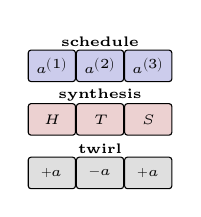
\begin{tikzpicture}[scale=0.68,
        box/.style={draw,rounded corners=1pt,minimum width=6mm,
                    minimum height=4mm,inner sep=1pt,font=\tiny}]
      % scheduling
      \node[font=\tiny\bfseries] at (0.9,2.55) {schedule};
      \node[box,fill=calblue!25] at (0,2.1) {$a^{(1)}$};
      \node[box,fill=calblue!25] at (0.9,2.1) {$a^{(2)}$};
      \node[box,fill=calblue!25] at (1.8,2.1) {$a^{(3)}$};
      % synthesis
      \node[font=\tiny\bfseries] at (0.9,1.55) {synthesis};
      \node[box,fill=mustred!20] at (0,1.1) {$H$};
      \node[box,fill=mustred!20] at (0.9,1.1) {$T$};
      \node[box,fill=mustred!20] at (1.8,1.1) {$S$};
      % twirl
      \node[font=\tiny\bfseries] at (0.9,0.55) {twirl};
      \node[box,fill=gray!25] at (0,0.1) {$+a$};
      \node[box,fill=gray!25] at (0.9,0.1) {$-a$};
      \node[box,fill=gray!25] at (1.8,0.1) {$+a$};
    \end{tikzpicture}
  \end{column}
  \end{columns}
  \cn{三种机制都会把一个角度打散：schedule 把它分到 $r$ 轮，synthesis 把它变成一串 Clifford$+T$ 字母，twirling 再给每个旋转乘上随机符号。}
  \vspace{-2mm}

  \begin{mustanswer}
    \footnotesize
    The bound is carried by the \alert{schedule alone}. Sign normalization is
    a bijection of the residue alphabet, so the standard \alert{folded
    (compile-time)} presentation inherits the bound verbatim.
    \alert{Nothing depends on tracking Pauli frames.}
    \cn{界只由 schedule 承担。符号归一化是残数字母表上的双射，所以标准的 folded（编译期）写法逐字继承这个界，完全不依赖追踪 Pauli frame。}
  \end{mustanswer}
\end{frame}

% ---------------------------------------------------------------- Frame 0.7
\begin{frame}{\bl{Where the compiler sits: downstream}%
                {编译器的位置：在下游}}
  \zhsub{编译器的位置：在下游}
  \centering
  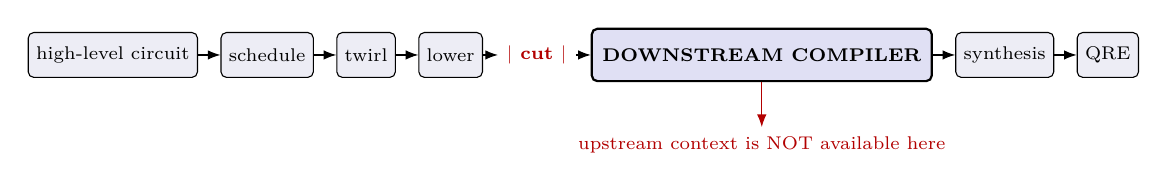
\begin{tikzpicture}[scale=0.95,transform shape,
      node distance=3mm,
      st/.style={draw,rounded corners=2pt,fill=softgrey,font=\scriptsize,
                 minimum height=6mm,inner xsep=3pt},
      big/.style={draw,thick,rounded corners=2pt,fill=calblue!15,
                  font=\scriptsize\bfseries,minimum height=7mm,inner xsep=4pt},
      ar/.style={-{Latex[length=1.6mm]},thin}]
    \node[st] (a) {high-level circuit};
    \node[st,right=of a] (b) {schedule};
    \node[st,right=of b] (c) {twirl};
    \node[st,right=of c] (d) {lower};
    \node[right=2mm of d,font=\scriptsize\bfseries,red!70!black] (cut) {$\rvert$ cut $\rvert$};
    \node[big,right=2mm of cut] (e) {DOWNSTREAM COMPILER};
    \node[st,right=of e] (f) {synthesis};
    \node[st,right=of f] (g) {QRE};
    \foreach \x/\y in {a/b,b/c,c/d,e/f,f/g} \draw[ar] (\x)--(\y);
    \draw[ar] (d)--(cut); \draw[ar] (cut)--(e);
    \draw[ar,red!70!black] (e.south) -- ++(0,-6mm)
      node[below,font=\scriptsize,align=center]
      {upstream context is \alert{NOT} available here};
  \end{tikzpicture}
  \medskip

  {\footnotesize Three real instances:
  \begin{itemize}\footnotesize
    \item a cloud transpiler receiving a flat QASM/QIR program without the
          user's high-level intent;
    \item a real-time stream optimizer inside the classical control stack;
    \item a vendor-side pass post-processing an already emitted instruction
          stream.
  \end{itemize}}
  \smallskip

  \begin{callout}
    If the compiler can see the circuit before randomization and lowering, the
    theorems do not apply --- and that boundary is itself the content of the
    design rule.
    \cn{若编译器能在 randomization 和 lowering 之前看到电路，定理就不适用——而这条边界本身就是设计规则的内容。}
  \end{callout}
  \note{先把这个位置立牢，否则后面所有质疑都会退化成"我为什么不能看上游"。
        答案：我们讨论的正是看不到上游的那一类编译器，而"要不要让它看到上游"
        本身就是设计规则的内容。}
\end{frame}

% ---------------------------------------------------------------- Frame 0.8
\begin{frame}{\bl{Also worth knowing (rapid fire)}{顺带一提（快速扫过）}}
  \zhsub{顺带一提（快速扫过）}
  \footnotesize
  \begin{itemize}
    \item \hd{fidelity} --- a closeness measure for states/operations;
          \emph{not used here}, we use operator-norm distances because they
          satisfy the triangle inequality (needed for packing arguments).
    \item \hd{oracle} --- a black-box subroutine charged per call; appears only
          in scope statements (``an uncharged random-access input oracle would
          be a different model'').
    \item \hd{FPGA / control stack} --- the classical electronics adjacent to
          the chip must resolve corrections \emph{before the next non-Clifford
          operation}, under hard latency and buffer budgets.
          \alert{This is why the bounded-memory streaming model is an
          engineering constraint, not a mathematical convenience.}
    \item \hd{spacetime volume} --- physical qubits $\times$ time
          (qubit-seconds).
    \item \hd{QRE} --- quantum resource estimator: logical circuit $+$
          architecture assumptions $\mapsto$ $T$ count, physical qubits,
          cycles, factories.
    \item \hd{lowering / IR / transpiler} --- lowering produces a \emph{flat
          instruction stream}; the graph/table the compiler keeps internally is
          the \emph{IR}.
    \item \hd{QAOA cost layer} --- $e^{-i\gamma C}$,
          $C=\sum_j w_jZ_{u_j}Z_{v_j}$: one $R_{ZZ}$ per edge.
  \end{itemize}
  \cn{这一页只需记住两点：我们用算子范数而不是 fidelity（因为 packing 论证需要三角不等式）；有界内存的流式模型来自工程约束算，不是数学上的方便假设。}
\end{frame}

% ---------------------------------------------------------------- Frame 0.9
\begin{frame}{\bl{Mathematical toolkit (1/2): circle distance}%
                {数学工具（1/2）：圆周距离}}
  \zhsub{数学工具（1/2）：圆周距离}
  \small
  \[
    \cd{u}:=\min_{k\in\mathbb{Z}}|u-2\pi k|\in[0,\pi],
    \qquad
    d_\circ(\alpha,\beta):=\cd{\alpha-\beta}.
  \]
  $d_\circ$ is a metric on $\mathbb{R}/2\pi\mathbb{Z}$ (the triangle
  inequality holds). The identity used throughout:
  \begin{equation}
    \boxed{\ |e^{iu}-1|=2\sin\big(\cd{u}/2\big).\ }\tag{0.1}
  \end{equation}
  \cn{$\cd\cdot$ 是圆周距离，已经把"绕过 $2\pi$"放进定义。$(0.1)$ 把弦长换算成角度。}
  \medskip

  {\scriptsize\hd{Verification.} $|e^{iu}-1|=2|\sin(u/2)|$; for
  $u\in[0,\pi]$, $\cd u=u$; for $u\in[\pi,2\pi]$, $\cd u=2\pi-u$ and
  $2\sin\!\big(\tfrac{2\pi-u}{2}\big)=2\sin\!\big(\pi-\tfrac u2\big)
   =2\sin\tfrac u2$.}
\end{frame}

% ---------------------------------------------------------------- Frame 0.10
\begin{frame}{\bl{Mathematical toolkit (2/2): four information-theoretic facts}%
                {数学工具（2/2）：四个信息论事实}}
  \zhsub{数学工具（2/2）：四个信息论事实}
  \scriptsize
  \hd{Prefix-free code}: no codeword is a prefix of another; concatenations
  are uniquely parseable without out-of-band lengths. All five serialization
  fields of the model are such codes.
  \smallskip

  \begin{columns}[T,onlytextwidth]
  \begin{column}{0.48\textwidth}
    \hd{Fact K (Kraft).} $\sum_i2^{-\ell_i}\le1$, hence
    \[ N\cdot2^{-\max_i\ell_i}\le1\ \Longrightarrow\ \max_i\ell_i\ge\log_2N. \]
    \emph{Proof (one line).} Map codeword $w$ to the dyadic interval
    $I_w=[0.w,\,0.w+2^{-|w|})$; $w$ is a prefix of $w'$ iff
    $I_{w'}\subseteq I_w$; prefix-freeness $\Rightarrow$ the $I_i$ are
    pairwise disjoint $\Rightarrow\sum2^{-\ell_i}=\sum|I_i|\le1$.
    \smallskip

    \hd{Fact S (Shannon).} Any prefix-free code satisfies
    $\mathbb{E}|E(X)|\ge H(X)$.
  \end{column}
  \begin{column}{0.48\textwidth}
    \hd{Fact F (Fano).} If $\hat X=f(Y)$ and $\Pr[\hat X\ne X]\le\delta$, then
    \[ H(X\mid Y)\le \hbin(\delta)+\delta\log_2(|\mathcal X|-1). \]
    \emph{Intuition (this is the proof skeleton):} given $Y$, to finish
    describing $X$ you need only say (i) did the guess fail ---
    $\hbin(\delta)$ bits; (ii) if so, which of the other $|\mathcal X|-1$
    values --- on average $\delta\log_2(|\mathcal X|-1)$ bits.
    \smallskip

    \hd{Corollary F$'$ (the only form used).} For $X$ uniform on
    $\mathcal X$:
    \[ I(X;Y)\ \ge\ (1-\delta)\log_2|\mathcal X|-\hbin(\delta). \]
  \end{column}
  \end{columns}
  \smallskip

  With $|\mathcal X|=K^m$:
  \begin{equation}
    \boxed{\ \Ldelta:=(1-\delta)\,m\log_2K-\hbin(\delta).\ }\tag{0.2}
  \end{equation}
  \cn{Kraft 给出"最长码字至少 $\log_2N$ 比特"；Fano 给出"能以 $\delta$ 错误率猜中，就意味着互信息足够大"。$(0.2)$ 是后面所有下界的右端。}
  \note{$(0.1)$ 和 $(0.2)$ 是全场引用最多的两个式子，编号必须显式打出来，
        后面所有帧都引用这两个编号。Fano 只用推论 F$'$ 这一种形式。}
\end{frame}

%%%%%%%%%%%%%%%%%%%%%%%%%%%%%%%%%%%%%%%%%%%%%%%%%%%%%%%%%%%%%%%%%%%%%%%%%%%%%%
%  PART II  ==  §1   Packing
%%%%%%%%%%%%%%%%%%%%%%%%%%%%%%%%%%%%%%%%%%%%%%%%%%%%%%%%%%%%%%%%%%%%%%%%%%%%%%
\section[\bl{1. Packing}{1. Packing}]{\bl{Packing: why distinguishable settings are countable}%
             {Packing：为什么"可区分的设置"有可数个}}

% ---------------------------------------------------------------- Frame 1.1
\begin{frame}{\bl{The projective distance, and why}{投影距离，以及为什么用它}}
  \zhsub{投影距离，以及为什么用它}
  \small
  \begin{defn}[projective distance]
    $\displaystyle \dproj(U,V):=\inf_{\varphi\in\mathbb{R}}
       \big\|U-e^{i\varphi}V\big\|_\op .$
  \end{defn}
  \begin{itemize}\footnotesize
    \item \hd{Infimum attained}: $\varphi\mapsto\|U-e^{i\varphi}V\|_\op$ is
          continuous on the compact circle $\{e^{i\varphi}\}\cong S^1$.
    \item \hd{Why quotient the global phase}: $U$ and $e^{i\varphi}U$ are
          physically indistinguishable. Without the quotient we would count
          physically identical objects as distinct, and \alert{the packing
          count would simply be wrong}.
  \end{itemize}
  \pause
  \begin{claim}[reduction to the relative unitary]
    $\displaystyle \dproj(U,V)=\inf_\varphi\big\|UV^\dagger-e^{i\varphi}I
      \big\|_\op .$
  \end{claim}
  \begin{prf}\footnotesize
    $\|AB\|_\op=\|A\|_\op$ for unitary $B$; take $B=V^\dagger$.
  \end{prf}
  \pause
  \begin{callout}
    The problem is now purely geometric: \alert{given the spectrum of a
    unitary (a set of points on the unit circle), rotate the whole circle to
    sit as close to $1$ as possible --- how far is the worst point?}
    \cn{问题现在纯粹是几何的：给定一个 unitary 的谱（单位圆上一组点），整体旋转让它尽量靠近 1 —— 最远的那个点还有多远？}
  \end{callout}
  \note{Claim 1.2 把两个酉算子的比较化成一个酉算子的谱几何问题。
        之后所有计算都在单位圆上进行。}
\end{frame}

% ---------------------------------------------------------------- Frame 1.3
\begin{frame}{\bl{Lemma 1.3: the two-point bound, and where the ``4'' comes from}%
                {引理 1.3：两点界，以及"4"从哪来}}
  \zhsub{引理 1.3：两点界，以及"4"从哪来}
  \begin{columns}[T,onlytextwidth]
  \begin{column}{0.60\textwidth}
    \scriptsize
    \begin{lemma2}[two-point bound]
      Let $\alpha,\beta\in\mathbb{R}/2\pi\mathbb{Z}$ with
      $d_\circ(\alpha,\beta)=\gamma\in[0,\pi]$. Then
      \[ \forall\varphi:\quad
         \max\big(|e^{i\alpha}-e^{i\varphi}|,\,|e^{i\beta}-e^{i\varphi}|\big)
         \ \ge\ 2\sin(\gamma/4), \]
      with equality when $\varphi$ is the \emph{midpoint of the short arc}
      between $\alpha$ and $\beta$.
    \end{lemma2}
  \cn{圆上两点相距 $\gamma$ 时，无论把全局相位转到哪里，总有一点离它至少 $2\sin(\gamma/4)$；取短弧中点时取等号。}
    \begin{prf}\tiny
      Triangle inequality on $d_\circ$:
      $d_\circ(\alpha,\varphi)+d_\circ(\varphi,\beta)\ge\gamma
       \Rightarrow\max\big(d_\circ(\alpha,\varphi),d_\circ(\beta,\varphi)
       \big)\ge\gamma/2$.
      WLOG $d_\circ(\alpha,\varphi)\ge\gamma/2$. By $(0.1)$,
      $|e^{i\alpha}-e^{i\varphi}|=2\sin\big(d_\circ(\alpha,\varphi)/2\big)$;
      since $t\mapsto2\sin(t/2)$ increases on $[0,\pi]$ and
      $d_\circ\in[0,\pi]$,
      $|e^{i\alpha}-e^{i\varphi}|\ge2\sin\big((\gamma/2)/2\big)
       =2\sin(\gamma/4)$.
      Equality: the short-arc midpoint gives
      $d_\circ(\alpha,\varphi)=d_\circ(\beta,\varphi)=\gamma/2$, and both
      chords equal $2\sin(\gamma/4)$.
    \end{prf}
  \end{column}
  \begin{column}{0.38\textwidth}
    \centering
    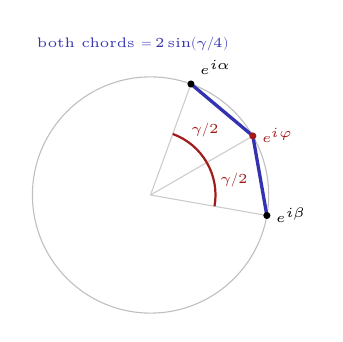
\begin{tikzpicture}[scale=1.5]
      \draw[gray!50] (0,0) circle (1);
      \coordinate (O) at (0,0);
      \coordinate (A) at (70:1);
      \coordinate (B) at (-10:1);
      \coordinate (M) at (30:1);
      \draw[gray!40] (O)--(A); \draw[gray!40] (O)--(B);
      \draw[gray!40] (O)--(M);
      \draw[very thick,calblue] (A)--(M);
      \draw[very thick,calblue] (B)--(M);
      \draw[mustred,thick] (70:0.55) arc (70:30:0.55);
      \draw[mustred,thick] (30:0.55) arc (30:-10:0.55);
      \node[font=\tiny,mustred] at (50:0.72) {$\gamma/2$};
      \node[font=\tiny,mustred] at (10:0.72) {$\gamma/2$};
      \fill (A) circle (0.03) node[above right,font=\tiny] {$e^{i\alpha}$};
      \fill (B) circle (0.03) node[right,font=\tiny] {$e^{i\beta}$};
      \fill[mustred] (M) circle (0.03)
        node[right,font=\tiny] {$e^{i\varphi}$};
      \node[font=\tiny,calblue,align=center] at (-0.15,1.28)
        {both chords $=2\sin(\gamma/4)$};
    \end{tikzpicture}
  \end{column}
  \end{columns}
  \smallskip

  \begin{mustanswer}[\bl{Why $\sin(\Theta/4)$ and not $\sin(\Theta/2)$?}%
                       {为什么是 $\sin(\Theta/4)$}]
    \footnotesize Two factors of $2$ compose:
    \textbf{(i)} the optimal global phase sits \alert{in the middle}
    $\Rightarrow$ angular distance halves from $\gamma$ to $\gamma/2$;
    \textbf{(ii)} the chord formula $|e^{iu}-1|=2\sin(u/2)$ carries a $/2$ of
    its own. \quad $\gamma/2$ then $/2$ gives $\gamma/4$.
    \cn{两个 2 叠加：最优全局相位落在中点，角距离从 $\gamma$ 减半到 $\gamma/2$；弦长公式又自带一个 $/2$。}
  \end{mustanswer}
\end{frame}

% ---------------------------------------------------------------- Frame 1.4
\begin{frame}{\bl{Lemma 1.4: the character surjectivity lemma}%
                {引理 1.4：特征标满射引理}}
  \zhsub{引理 1.4：特征标满射引理}
  \small
  \begin{lemma2}[character surjectivity]
    For $a_1,\dots,a_m\in\Fb^n$:
    \[ a_1,\dots,a_m\ \text{linearly independent over }\Fb
       \iff
       \Phi:\Fb^n\to\{\pm1\}^m,\
       z\mapsto\big(\chi_{a_1}(z),\dots,\chi_{a_m}(z)\big)\
       \text{surjective}. \]
  \end{lemma2}
  \cn{$a_j$ 在 $\Fb$ 上线性无关，等价于这些 character 联合起来能取遍 $\{\pm1\}^m$ 的每一种符号模式。}
  \begin{prf}\footnotesize
    Let $A\in\Fb^{m\times n}$ have rows $a_j$ and $L(z)=Az$. The map
    $\Fb^m\to\{\pm1\}^m$, $(b_j)\mapsto((-1)^{b_j})$, is a bijection, and
    $\Phi=(-1)^{L(\cdot)}$. Hence
    $\Phi\ \text{surjective}\iff L\ \text{surjective}
     \iff\operatorname{rank}A=m\iff\text{rows independent}$.
  \end{prf}
  \pause
  \begin{callout}
    This is the entire group-theoretic content --- and the origin of the
    paper's \alert{most attackable assumption}. Lose $\Fb$-independence and
    $\Phi$ is no longer surjective; the very first step of Theorem 1.7 below
    cannot be executed, and the coefficients are no longer identifiable.
    \cn{这就是全部的群论内容，也是全文最容易被攻击的假设。失去 $\Fb$-无关性，$\Phi$ 不再满射，Theorem 1.7 的第一步就执行不了，系数也不再可辨识。}
  \end{callout}
  \note{scope 伏笔：$\Fb$-无关性是最容易被攻击的假设。
        主动指出它，并说明失去它之后坏掉的是 Theorem 1.7 的第一步
        （选 $z,z'$ 那一步），而不是别的地方。}
\end{frame}

% ---------------------------------------------------------------- Frame 1.5
\begin{frame}{\bl{Definitions: wrap margin and the phase family}%
                {定义：绕转裕度与相位族}}
  \zhsub{定义：绕转裕度与相位族}
  \small
  \begin{defn}[wrap margin]
    For alphabet $[K]_0=\{0,\dots,K-1\}$, $K\ge2$, step $\Delta>0$:
    \[ \gamma(K,\Delta):=\min_{1\le d\le K-1}\cd{d\Delta}. \]
  \cn{wrap margin：两个系数最少能差多少角度。$\cd\cdot$ 已经把绕转算进去了。}
  \end{defn}
  ``The least angle by which two coefficients can differ'' --- and $\cd\cdot$
  already accounts for wrapping past $2\pi$.
  \smallskip
  \pause

  \begin{defn}[phase family]
    $P_j=Z^{a_j}$ with $a_1,\dots,a_m$ $\Fb$-independent,
    \[ U_x:=\exp\Big(-\tfrac i2\sum_{j=1}^m x_j\Delta P_j\Big),
       \qquad x\in[K]_0^m . \]
  \cn{相位族：每个坐标 $x_j$ 取自 $K$ 元字母表，乘上步长 $\Delta$ 作为 $P_j$ 的转角，共 $K^m$ 个目标。}
  \end{defn}
  \note{两个定义都很短，但 $\gamma(K,\Delta)$ 里的 $\cd\cdot$ 是关键：
        它把"绕过 $2\pi$"这件事直接吸收进定义，不需要主值假设。}
\end{frame}

% ---------------------------------------------------------------- Frame 1.6
\begin{frame}{\bl{Theorem 1.7: exact worst-pair separation}%
                {定理 1.7：最坏点对的精确分离}}
  \zhsub{定理 1.7：最坏点对的精确分离}
  \scriptsize
  \begin{theorem}[exact separation]
    For every $m\ge1$,
    \[ \boxed{\ \min_{x\ne y}\dproj(U_x,U_y)
       =2\sin\!\Big(\frac{\gamma(K,\Delta)}{4}\Big).\ } \]
    In particular the family is projectively injective
    $\iff\gamma(K,\Delta)>0$.
    \cn{最坏点对的投影距离精确等于 $2\sin(\gamma(K,\Delta)/4)$；该族投影单射当且仅当 $\gamma(K,\Delta)>0$。}
  \end{theorem}
  \vspace{1mm}
  \pause
  \tiny
  \begin{prf}[Proof, direction $(\ge)$]
    Take $x\ne y$, $s:=x-y\ne0$, pick $j^*$ with $s_{j^*}\ne0$. By Claim 1.2
    consider
    \[ W:=U_xU_y^\dagger=\exp\Big(-\tfrac{i\Delta}2\sum_j s_jP_j\Big),\quad
       W|z\rangle=\lambda(z)|z\rangle,\quad
       \lambda(z)=\exp\Big(-\tfrac{i\Delta}2\sum_j s_j\chi_{a_j}(z)\Big). \]
    By Lemma 1.4, $\Phi$ is surjective, so choose $z,z'$ with
    $\chi_{a_j}(z)=\chi_{a_j}(z')$ for $j\ne j^*$, and
    $\chi_{a_{j^*}}(z)=+1$, $\chi_{a_{j^*}}(z')=-1$. Then
    \[ \arg\lambda(z)-\arg\lambda(z')
       =-\tfrac\Delta2\big(s_{j^*}-(-s_{j^*})\big)=-\Delta s_{j^*}
       \ \Longrightarrow\
       d_\circ\big(\arg\lambda(z),\arg\lambda(z')\big)
       =\cd{\Delta s_{j^*}}\ \ge\ \gamma(K,\Delta), \]
    since $1\le|s_{j^*}|\le K-1$. Finally
    $\|W-e^{i\varphi}I\|_\op=\max_z|\lambda(z)-e^{i\varphi}|
     \ge\max\big(|\lambda(z)-e^{i\varphi}|,|\lambda(z')-e^{i\varphi}|\big)$,
    so taking $\inf_\varphi$ and applying Lemma 1.3 gives
    $\dproj(U_x,U_y)\ge2\sin(\gamma/4)$.
  \end{prf}
  \pause
  \begin{prf}[Proof, direction $(\le)$: equality is attained]
    Pick $d\in\{1,\dots,K-1\}$ attaining $\gamma$ and take $x-y=d\,e_{j^*}$.
    Then $\sum_js_j\chi_{a_j}(z)=d\,\chi_{a_{j^*}}(z)\in\{+d,-d\}$, so the
    spectrum of $W$ is \alert{exactly two points} $\{e^{\mp i\Delta d/2}\}$ at
    circle distance $\cd{\Delta d}=\gamma$. Lemma 1.3's equality case gives
    $\inf_\varphi=2\sin(\gamma/4)$.
  \end{prf}
\end{frame}

% ---------------------------------------------------------------- Frame 1.7
\begin{frame}{\bl{Corollaries 1.8/1.9: both regimes give $\gamma=\Delta$}%
                {推论 1.8/1.9：两种算术区间都给出 $\gamma=\Delta$}}
  \zhsub{推论 1.8/1.9：两种算术区间都给出 $\gamma=\Delta$}
  \small
  \begin{block}{Corollary 1.8}\footnotesize
    \begin{enumerate}
      \item \hd{no-wrap regime}: if $(K-1)\Delta\le\pi$ then for all
            $1\le d\le K-1$, $d\Delta\in[\Delta,\pi]$, so
            $\cd{d\Delta}=d\Delta\ge\Delta$ and $\gamma=\Delta$.
      \item \hd{cyclic regime}: if $\Delta=2\pi/Q$ and $K\le Q-1$ then
            $\cd{d\Delta}=(2\pi/Q)\min(d,Q-d)\ge2\pi/Q=\Delta$, so
            $\gamma=\Delta$.
    \end{enumerate}
  \end{block}
  \begin{block}{Corollary 1.9 (uniform separation)}\footnotesize
    In both regimes
    \[ \min_{x\ne y}\dproj(U_x,U_y)=2\sin(\Delta/4), \]
    i.e.\ the $K^m$ targets form a \alert{packing} of separation
    $2\sin(\Delta/4)$.
  \end{block}
  \pause
  \begin{callout}
    In the cyclic regime the coefficient interval
    $[0,(Q-2)\cdot2\pi/Q]$ \alert{may cross $\pi$}. A textbook
    principal-value argument on $[-\pi,\pi]$ would go wrong here. Theorem 1.7
    handles wraparound exactly via $\cd\cdot$, needing no principal-interval
    hypothesis. \alert{This is the entire meaning of ``exact wrap margin.''}
    \cn{cyclic 情形下系数区间可能越过 $\pi$，教科书式的主值论证在这里会出错。Theorem 1.7 用 $\cd\cdot$ 精确处理绕转，不需要主值假设——这就是"精确 wrap margin"的全部含义。}
  \end{callout}
  \note{"合"在这里：两种区间制度殊途同归到 $\gamma=\Delta$。
        并且要主动说明为什么不能用教科书的主值论证——cyclic 区间会越过 $\pi$。}
\end{frame}

% ---------------------------------------------------------------- Frame 1.8
\begin{frame}{\bl{Lemma 1.10: from packing to a decoder (the pivot)}%
                {引理 1.10：从 packing 到译码器（枢纽）}}
  \zhsub{引理 1.10：从 packing 到译码器（枢纽）}
  \small
  \begin{lemma2}[nearest-packing decoder]
    If $\mathcal F=\{U_x\}_{x\in\mathcal X}$ is pairwise
    $\dproj\ge4\varepsilon$ and
    $\hat x(C):=\arg\min_y\dproj(U(C),U_y)$ (fixed tie rule), then
    \[ \dproj(U(C),U_x)\le\varepsilon\ \Longrightarrow\ \hat x(C)=x. \]
    \cn{若族两两分离 $\ge4\varepsilon$，则最近邻 packing 译码器能从任何 $\varepsilon$-正确的输出唯一恢复 $x$。}
  \end{lemma2}
  \begin{prf}\footnotesize
    For $y\ne x$:
    $\dproj(U(C),U_y)\ge\dproj(U_x,U_y)-\dproj(U_x,U(C))
     \ge4\varepsilon-\varepsilon=3\varepsilon>\varepsilon
     \ge\dproj(U(C),U_x)$.
  \end{prf}
  \pause
  \begin{mustanswer}[\bl{The pivot of the entire paper}{全文的枢纽}]
    It converts the soft statement \emph{``the compiler's output is
    correct''} into the hard statement \emph{``the output uniquely determines
    $x$''}. Hence \alert{any correct compiler is forced to encode all of $x$
    somewhere in its output} --- and information can be counted in bits.
    Part V does nothing but apply this conversion three times.
    \cn{这条引理是全文的枢纽：把"编译器输出正确"这句软话，变成"输出唯一确定 $x$"这句硬话。于是任何正确的编译器都被迫在输出里编码整个 $x$，而信息可以用比特来数。}
  \end{mustanswer}
\end{frame}

%%%%%%%%%%%%%%%%%%%%%%%%%%%%%%%%%%%%%%%%%%%%%%%%%%%%%%%%%%%%%%%%%%%%%%%%%%%%%%
%  PART III  ==  §2   Calibration
%%%%%%%%%%%%%%%%%%%%%%%%%%%%%%%%%%%%%%%%%%%%%%%%%%%%%%%%%%%%%%%%%%%%%%%%%%%%%%
\section[\bl{2. Calibration}{2. Calibration}]%
        {\texorpdfstring{\bl{Calibration: $K_\varepsilon$ was not chosen by me}%
                            {Calibration：$K_\varepsilon$ 不是专门构造的}}%
                        {\bl{Calibration: K_eps was not chosen by me}%
                            {Calibration: K_eps 不是专门构造的}}}

% ---------------------------------------------------------------- Frame 2.1
\begin{frame}{\bl{The question, stated as an objection}{把质疑先说出来}}
  \zhsub{把质疑先说出来}
  \vfill
  \begin{center}
  \begin{minipage}{0.84\textwidth}
    \begin{block}{}
      \large
      \emph{``Isn't $K$ chosen to make the bound look good?''}
      \bigskip

      \alert{No:} $K_\varepsilon$ equals the metric-entropy count of pairwise
      distinguishable rotations at tolerance $\varepsilon$, up to an
      explicitly interpretable factor.
    \end{block}
  \end{minipage}
  \end{center}
  \vfill
\end{frame}

% ---------------------------------------------------------------- Frame 2.2
\begin{frame}{\bl{Definitions and the exact single-axis distance}%
                {定义与单轴精确距离}}
  \zhsub{定义与单轴精确距离}
  \small
  \begin{defn}
    $g_\varepsilon:=4\arcsin(2\varepsilon)$, and
    \[ N(\varepsilon):=\max\big\{|S|:S\subseteq
       \{R_P(\theta)\}_{\theta\in\mathbb{R}/2\pi\mathbb{Z}},\
       \text{pairwise }\dproj\ge4\varepsilon\big\}. \]
  \end{defn}
  \pause
  \begin{lemma2}
    $\dproj\big(R_P(\theta),R_P(\theta')\big)=2\sin(g/4)$ where
    $g:=d_\circ(\theta,\theta')$.
  \end{lemma2}
  \begin{prf}\footnotesize
    $R_P(\theta)R_P(\theta')^\dagger=R_P(\delta)$, $\delta=\theta-\theta'$,
    whose spectrum is exactly the two points $e^{\mp i\delta/2}$ at circle
    distance $\cd\delta=g$; apply the equality case of Lemma 1.3.
  \end{prf}
  \pause
  \begin{block}{Corollary 2.3}\footnotesize
    pairwise $\dproj\ge4\varepsilon$ $\iff$ pairwise
    $d_\circ\ge g_\varepsilon$, because
    $2\sin(g_\varepsilon/4)=2\sin(\arcsin2\varepsilon)=4\varepsilon$
    \alert{exactly} --- that is how $g_\varepsilon$ was defined.
  \end{block}
  \note{$g_\varepsilon$ 的定义是为了让 Corollary 2.3 成为恒等式而不是估计。
        这一点后面 Corollary 2.5 会直接变现。}
\end{frame}

% ---------------------------------------------------------------- Frame 2.3
\begin{frame}{\bl{Theorem 2.4 and the cyclic exact identity}%
                {定理 2.4 与 cyclic 情形的恒等}}
  \zhsub{定理 2.4 与 cyclic 情形的恒等}
  \small
  \begin{theorem}[metric-entropy count]
    \[ N(\varepsilon)=\Big\lfloor\frac{2\pi}{g_\varepsilon}\Big\rfloor,
       \qquad \frac1{2\varepsilon}-1<N(\varepsilon)\le\frac\pi{4\varepsilon}. \]
    \cn{容差 $\varepsilon$ 下两两可区分的旋转个数恰为 $\lfloor2\pi/g_\varepsilon\rfloor$，夹在 $1/2\varepsilon-1$ 与 $\pi/4\varepsilon$ 之间。}
  \end{theorem}
  \begin{prf}\footnotesize
    On a circle of circumference $2\pi$, points pairwise $\ge g$ apart number
    at most $\lfloor2\pi/g\rfloor$ (order them; the gaps sum to $2\pi$ and
    each is $\ge g$), attained by equal spacing. The two-sided estimate uses
    $x\le\arcsin x\le\frac\pi2x$ on $[0,1]$:
    $g_\varepsilon\in[8\varepsilon,4\pi\varepsilon]$.
  \end{prf}
  \pause
  \begin{block}{Corollary 2.5 (cyclic: exact equality)}\footnotesize
    The paper takes
    $Q_\varepsilon:=\big\lfloor\frac\pi{2\arcsin2\varepsilon}\big\rfloor$, and
    \[ \frac\pi{2\arcsin2\varepsilon}=\frac{2\pi}{4\arcsin2\varepsilon}
       =\frac{2\pi}{g_\varepsilon}
       \ \Longrightarrow\ \boxed{\,Q_\varepsilon=N(\varepsilon)\,}. \]
  \end{block}
  \begin{callout}
    The sharing modulus equals the metric-entropy count itself --- no free
    parameter at all.
    \cn{sharing modulus 恰好等于 metric-entropy 计数本身——一个自由参数都没有。}
  \end{callout}
\end{frame}

% ---------------------------------------------------------------- Frame 2.4
\begin{frame}{\bl{Proposition 2.6: what the factor $4$ is}%
                {命题 2.6：那个因子 4 到底是什么}}
  \zhsub{命题 2.6：那个因子 4 到底是什么}
  \scriptsize
  \begin{prop2}
    With $L_\varepsilon=\lfloor\frac\pi{8\arcsin2\varepsilon}\rfloor$,
    $K_\varepsilon=L_\varepsilon+1$,
    $\Delta_\varepsilon=\frac\pi{2L_\varepsilon}$:
    \[ (K_\varepsilon-1)\Delta_\varepsilon
       =L_\varepsilon\cdot\frac\pi{2L_\varepsilon}=\frac\pi2\le\pi
       \quad(\text{no-wrap holds}),
       \qquad
       \frac{\Delta_\varepsilon}4=\frac\pi{8L_\varepsilon}
       \ge\arcsin2\varepsilon
       \ \Longrightarrow\ 2\sin(\Delta_\varepsilon/4)\ge4\varepsilon, \]
    and with $y:=\frac\pi{2\arcsin2\varepsilon}$ (so $N=\lfloor y\rfloor$,
    $K_\varepsilon=\lfloor y/4\rfloor+1$):
    $\displaystyle \frac{N(\varepsilon)}4<K_\varepsilon
      <\frac{N(\varepsilon)}4+\frac32 .$
  \end{prop2}
  \pause
  \begin{mustanswer}
    The factor $4$ is \alert{not slack in an estimate} --- it is exactly the
    price of the no-wrap condition restricting the coefficient range to the
    quarter period $[0,\pi/2]$. The cyclic version has no such restriction and
    degenerates to the exact identity $Q_\varepsilon=N(\varepsilon)$.
    \alert{Both directions are stated as two-sided bounds; no tighter constant
    is claimed.}
    \cn{因子 4 不是估计里的余量，而正是 no-wrap 条件把系数范围限制到四分之一周期 $[0,\pi/2]$ 的代价。两个方向都写成双边界，未声称更紧的常数。}
  \end{mustanswer}
  \note{最后半句"我们没有声称更紧的常数"要主动说出来，
        它挡掉一整类"常数是不是调出来的"追问。}
\end{frame}

% ---------------------------------------------------------------- Frame 2.5
\begin{frame}{\bl{Remark 2.7: why $\log(1/\varepsilon)$ appears twice}%
                {注 2.7：$\log(1/\varepsilon)$ 为什么出现两次}}
  \zhsub{注 2.7：$\log(1/\varepsilon)$ 为什么出现两次}
  \small
  Ross--Selinger guarantees that \alert{every} grid angle costs
  $\Theta(\log(1/\varepsilon))$ in Clifford$+T$ synthesis, \alert{uniformly
  over the alphabet}. Hence
  \[ \underbrace{m\log_2K_\varepsilon}_{\text{information side: alphabet size}}
     =m\log_2\Theta(1/\varepsilon),
     \qquad
     \underbrace{3\log_2(1/\varepsilon)}
       _{\text{physical side: repair cost per coordinate}} \]
  \pause
  \begin{callout}
    The two logarithms come from the \alert{same grid}. This --- not an
    analogy --- is the technical basis on which ``exchange rate'' is a
    legitimate word.
    \cn{两个对数来自同一个网格。它是"汇率"这个词在技术上成立的基础。}
  \end{callout}
\end{frame}

% ------------------------------------------------------------- Frame 2.5(b)
\begin{frame}{\bl{The exchange rate in miniature}{汇率缩影}}
  \zhsub{汇率缩影}
  \vfill
  \begin{center}
  \begin{minipage}{0.90\textwidth}
    \begin{block}{}
      \normalsize
      One QAOA cost layer, 3-regular MaxCut on 22 vertices:
      $m=33$ edges, $\varepsilon=10^{-3}$.
      \smallskip

      $L_\varepsilon=\lfloor\pi/(8\arcsin2\varepsilon)\rfloor=196$,
      \quad $K_\varepsilon=197$.
      \smallskip

      Per edge: $\log_2 197=7.62$ bits. \quad
      Whole layer: \alert{$252$ bits $\approx31$ bytes}.
      \bigskip

      A compiler that \hd{defers} carries those $31$ bytes across every cut.
      \smallskip

      A compiler that \hd{commits early} buys the same information back at
      $\approx3\log_2(1/\varepsilon)\approx30$ $T$ gates per corrected
      coordinate: \alert{order $10^3$ magic states.}
    \end{block}
  \end{minipage}
  \end{center}
  \vfill
\end{frame}

%%%%%%%%%%%%%%%%%%%%%%%%%%%%%%%%%%%%%%%%%%%%%%%%%%%%%%%%%%%%%%%%%%%%%%%%%%%%%%
%  PART IV  ==  §3   Dispersal
%%%%%%%%%%%%%%%%%%%%%%%%%%%%%%%%%%%%%%%%%%%%%%%%%%%%%%%%%%%%%%%%%%%%%%%%%%%%%%
\section[\bl{3. Dispersal}{3. Dispersal}]{\bl{Dispersal: no record leaks the aggregate}%
             {Dispersal：为什么没有记录泄露 aggregate}}

% ---------------------------------------------------------------- Frame 3.1
\begin{frame}{\bl{Definition 3.1: the $r$-round dispersed update stream}%
                {定义 3.1：$r$ 轮打散更新流}}
  \zhsub{定义 3.1：$r$ 轮打散更新流}
  \small
  \begin{defn}[dispersed stream]
    Fix $Q\ge3$, $\Delta=2\pi/Q$, $K=Q-1$, $r\ge2$.
    \hd{Semantic input}: $x\in[K]_0^m$ --- $m$ addressed records.
    \hd{Flat input}: round-major records $\mathrm{Update}(t,j,a_j^{(t)})$,
    $a_j^{(t)}\in\ZQ$, with
    \begin{equation}
      \sum_{t=1}^r a_j^{(t)}\equiv x_j\pmod Q,\qquad j\in[m],\tag{3.1}
    \end{equation}
    realizing
    $W=\prod_{t=1}^r\prod_{j=1}^m R_{P_j}\big(\Delta a_j^{(t)}\big)$.
    \cn{语义输入是 $m$ 个 aggregate；平坦输入是 round-major 的更新记录，每个坐标在 $r$ 轮上模 $Q$ 求和才等于 aggregate。}
  \end{defn}
  \vspace{-2mm}
  \begin{center}
  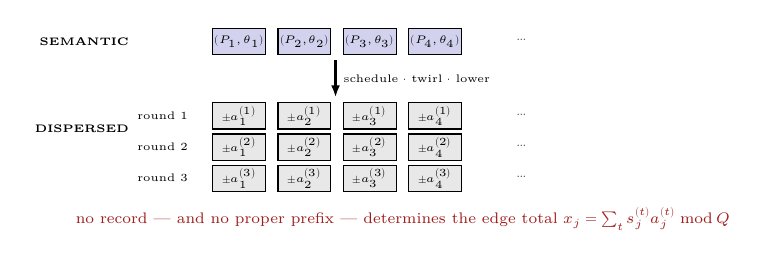
\begin{tikzpicture}[scale=0.79,transform shape,
      sq/.style={draw,minimum width=8.5mm,minimum height=4.2mm,
                 font=\tiny,inner sep=1pt},
      ar/.style={-{Latex[length=1.5mm]}}]
    % semantic row
    \node[font=\tiny\bfseries,anchor=east] at (-0.6,2.35) {SEMANTIC};
    \foreach \i in {1,2,3,4} {
      \node[sq,fill=calblue!22] at (\i*1.05,2.35)
        {$(P_{\i},\theta_{\i})$};}
    \node[font=\tiny] at (5.6,2.35) {$\cdots$};
    % arrow
    \draw[ar,thick] (2.6,2.05) -- (2.6,1.45)
      node[midway,right,font=\tiny] {schedule $\cdot$ twirl $\cdot$ lower};
    % dispersed rows
    \node[font=\tiny\bfseries,anchor=east] at (-0.6,0.95) {DISPERSED};
    \foreach \t/\y in {1/1.15,2/0.65,3/0.15} {
      \node[font=\tiny,anchor=east] at (0.35,\y) {round \t};
      \foreach \i in {1,2,3,4} {
        \node[sq,fill=gray!18] at (\i*1.05,\y) {$\pm a_{\i}^{(\t)}$};}
      \node[font=\tiny] at (5.6,\y) {$\cdots$};}
    \node[font=\scriptsize,anchor=west,mustred] at (-1.7,-0.5)
      {no record --- and no proper prefix --- determines the edge total
       $x_j=\sum_t s_j^{(t)}a_j^{(t)}\bmod Q$};
  \end{tikzpicture}
  \end{center}
\end{frame}

% ---------------------------------------------------------------- Frame 3.2
\begin{frame}{\bl{Correctness: Claim 3.2 $+$ Proposition 3.3}%
                {正确性：命题 3.2 与 3.3}}
  \zhsub{正确性：命题 3.2 与 3.3}
  \small
  \begin{claim}
    $R_P(\theta+2\pi k)=(-1)^kR_P(\theta)$.
  \end{claim}
  \begin{prf}\footnotesize
    $\exp(-i\pi P)$ acts as $e^{\mp i\pi}=-1$ on both $\pm1$ eigenspaces of
    $P$, so $\exp(-i\pi P)=-I$; iterate.
  \end{prf}
  \pause
  \begin{prop2}
    Any flat stream satisfying $(3.1)$ realizes $U_x$ up to a global phase.
  \end{prop2}
  \begin{prf}\footnotesize
    The $P_j$ commute, so
    $W=\prod_jR_{P_j}\big(\Delta\sum_ta_j^{(t)}\big)$. With integer
    representatives $\sum_ta_j^{(t)}=x_j+Qk_j$ and $Q\Delta=2\pi$, Claim 3.2
    gives $R_{P_j}(\Delta x_j+2\pi k_j)=(-1)^{k_j}R_{P_j}(\Delta x_j)$; the
    product of signs $(-1)^{\sum_jk_j}$ is global, and $\dproj$ has already
    quotiented it.
  \end{prf}
\end{frame}

% ---------------------------------------------------------------- Frame 3.3
\begin{frame}{\bl{Proposition 3.4: record and prefix privacy}%
                {命题 3.4：单记录与真前缀的隐私性}}
  \zhsub{命题 3.4：单记录与真前缀的隐私性}
  \small
  \begin{prop2}
    \begin{enumerate}\footnotesize
      \item For any fixed $(t,j,a)$ and any $b\in[K]_0$, there is a valid
            stream with $a_j^{(t)}=a$ \alert{and} $x_j=b$.
      \item Under the \hd{canonical sharing distribution} (first $r-1$ shares
            i.i.d.\ uniform on $\ZQ$, last fixed by $(3.1)$), every individual
            residue is uniform on $\ZQ$ \alert{and independent of $x_j$}.
      \item After any proper prefix, the final-round residue choice reaches
            every aggregate in $\ZQ^m$, hence every $x\in[K]_0^m$.
    \end{enumerate}
  \end{prop2}
  \begin{prf}\footnotesize
    (1) Since $r\ge2$, pick $t'\ne t$ and set
    $a_j^{(t')}:=b-a-\sum_{t''\ne t,t'}a_j^{(t'')}\bmod Q$.
    (2) For $r=2$: $a^{(1)}$ uniform; conditioning on $x_j$ leaves it uniform;
    $a^{(2)}=x_j-a^{(1)}$ is then uniform. A sum containing at least one
    independent uniform term is uniform.
    (3) Apply (1) coordinatewise.
  \end{prf}
  \pause
  \begin{callout}
    $(3.1)$ together with 3.4(2) \alert{is additive secret sharing over
    $\ZQ$} --- a one-time pad. Constructing a secret sharing is cheap and is
    \emph{not} the contribution. \alert{The contribution is the next slide.}
    \cn{$(3.1)$ 加上 3.4(2) 就是 $\ZQ$ 上的加法secret sharing，一次性密码本。构造secret sharing很便宜，不是贡献；贡献在下一帧。}
  \end{callout}
\end{frame}

% ---------------------------------------------------------------- Frame 3.4
\begin{frame}{\bl{Proposition 4: the FT stack emits these streams anyway}%
                {命题 4：容错栈本来就在发这种流}}
  \zhsub{命题 4：容错栈本来就在发这种流}
  \small
  Each of the following emits streams of Definition 3.1, and each generated
  family satisfies the hypotheses of the lower bounds:
  \begin{itemize}\footnotesize
    \item \hd{(a) Time-dependent Trotterization.} $H(t)=\sum_jc_j(t)P_j$ with
          step $\tau$; round $t$ applies $R_{P_j}(2c_j(t_t)\tau)$; grid
          rounding gives $a_j^{(t)}$, $s\equiv+1$.
    \item \hd{(b) Layerwise-parameterized phase layers.} A depth-$r$ ansatz
          whose round-$t$ commuting layer carries free coefficients
          $\theta_j^{(t)}$.
    \item \hd{(c) Randomized compiling of (a) or (b).} Twirling multiplies
          each residue by $s_j^{(t)}$, in folded or tracked mode.
  \end{itemize}
  \pause
  \begin{mustanswer}[\bl{The counterexample --- state it yourself}%
                       {反例，必须自己讲出来}]
    \footnotesize
    \alert{The constant schedule $a_j^{(t)}\equiv a_j$ is degenerate}:
    $x_j=ra_j\bmod Q$ is determined by round one alone.
    This is exactly why \alert{controlled-power ladders and phase estimation
    are OUT of scope}: they supply contiguity but \alert{not} coefficient
    freedom.
    An exhaustive enumeration at $(m,r,Q)=(2,2,5)$ confirms all three
    behaviours (frozen artifact \texttt{fooling\_set\_m2\_r2\_Q5.json}).
    \cn{常数 schedule 是退化的——第一轮就把 aggregate 定死了。所以 controlled-power ladder 和 phase estimation 明确不在范围内：它们提供 contiguity，但不提供跨轮次的系数自由度。}
  \end{mustanswer}
\end{frame}

% -------------------------------------------------------------- Frame 3.5(a)
\begin{frame}{\bl{Lemma 3.5: Clifford records normalize away}%
                {引理 3.5：Clifford 记录可以归一化掉}}
  \zhsub{引理 3.5：Clifford 记录可以归一化掉}
  \scriptsize
  \begin{lemma2}[Clifford interleaving]
    Suppose the rounds are separated by Clifford records and the accumulated
    Clifford $D_{t-1}$ satisfies
    \begin{equation}
      D_{t-1}^\dagger P_jD_{t-1}=\varepsilon_j^{(t)}P_{\pi_t(j)},
      \qquad \varepsilon_j^{(t)}\in\{\pm1\},\ \pi_t\in S_m.\tag{3.2}
    \end{equation}
    Then commuting every Clifford record to the end yields a stream of
    Definition 3.1 on the same generators (residues unchanged, signs
    multiplied by $\varepsilon_j^{(t)}$, coordinates relabelled by $\pi_t$),
    plus a fixed Clifford suffix $D_r$.
  \end{lemma2}
  \begin{prf}
    Write the emitted unitary as $D'_rL_r\cdots D'_1L_1$. Moving each Clifford
    leftwards replaces $L_t$ by $D_{t-1}^\dagger L_tD_{t-1}$; since
    conjugation is an automorphism and
    $L_t=\prod_jR_{P_j}(\Delta s_j^{(t)}a_j^{(t)})$, $(3.2)$ gives
    $D_{t-1}^\dagger L_tD_{t-1}
     =\prod_jR_{P_{\pi_t(j)}}\big(\Delta\varepsilon_j^{(t)}s_j^{(t)}
      a_j^{(t)}\big)$.
    $D_{t-1}$ --- hence $\pi_t,\varepsilon^{(t)}$ --- is computable from the
    prefix, so the normalization is \alert{prefix-measurable}; $D_r$ is common
    to the family and unitary, preserving projective distance and the
    separation of Theorem 1.7.
  \end{prf}
  \note{把 Clifford 记录一路交换到最后，得到的仍然是 Definition 3.1 的流：
        残数不变，符号乘上 $\varepsilon_j^{(t)}$，坐标被 $\pi_t$ 重标。
        关键词是 prefix-measurable——归一化可由前缀算出，不需要额外信息。}
\end{frame}

% -------------------------------------------------------------- Frame 3.5(b)
\begin{frame}{\bl{Corollary 3.6: nothing depends on Pauli frames}%
                {推论 3.6：不依赖 Pauli frame}}
  \zhsub{推论 3.6：不依赖 Pauli frame}
  \small
  \begin{block}{Corollary 3.6}
    $a\mapsto sa\bmod Q$ ($s=\pm1$) is a bijection of $\ZQ$ $\Rightarrow$ the
    twirled family maps \alert{record-for-record} onto the untwirled family,
    preserving aggregates, record boundaries and cut positions.
  \end{block}
  \pause
  \begin{mustanswer}[\bl{Nothing depends on Pauli frames --- and the boundary}%
                       {不依赖 Pauli frame——以及边界}]
    \footnotesize
    Sign normalization is a \alert{bijection of the residue alphabet}, so the
    standard folded (compile-time) presentation of randomized compiling
    inherits every bound verbatim.
    \alert{Boundary (state it before being asked):} $(3.2)$ is a real
    restriction. It holds for Pauli-frame layers ($\pi_t=\mathrm{id}$) and for
    routing/SWAP layers permuting the generating set. \alert{It fails} if some
    accumulated Clifford sends a $P_j$ to a \emph{product} of generators
    rather than a generator --- the rounds then accumulate in different bases
    and the coordinatewise structure is lost.
    \cn{符号归一化是残数字母表上的双射，folded 写法逐字继承所有界。边界要主动说：若某个累积 Clifford 把 $P_j$ 送到生成元的乘积而不是生成元，各轮就在不同基底上累加，坐标结构随之丢失。}
  \end{mustanswer}
  \note{"不依赖 Pauli frame"的全部内容都在这里。
        同时主动交出 $(3.2)$ 的边界：如果某个累积 Clifford 把 $P_j$ 送到
        生成元的乘积而不是生成元，坐标结构就没了。}
\end{frame}

%%%%%%%%%%%%%%%%%%%%%%%%%%%%%%%%%%%%%%%%%%%%%%%%%%%%%%%%%%%%%%%%%%%%%%%%%%%%%%
%  PART V  ==  §4   The lower bounds
%%%%%%%%%%%%%%%%%%%%%%%%%%%%%%%%%%%%%%%%%%%%%%%%%%%%%%%%%%%%%%%%%%%%%%%%%%%%%%
\section[\bl{4. Lower bounds}{4. 下界}]{\bl{The lower bounds: one argument, three variations}%
             {下界：一个论证的三次变奏}}

% ---------------------------------------------------------------- Frame 4.0
\begin{frame}{\bl{Roadmap: one argument, three variations}%
                {路线图：只有一个论证}}
  \zhsub{路线图：只有一个论证}
  \begin{columns}[T,onlytextwidth]
  \begin{column}{0.40\textwidth}
    \centering
    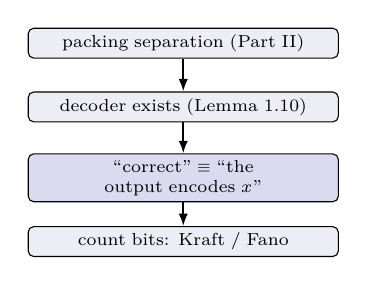
\begin{tikzpicture}[scale=0.9,transform shape,
        nd/.style={draw,rounded corners=2pt,fill=softgrey,font=\scriptsize,
                   text width=42mm,align=center,inner sep=2.5pt},
        ar/.style={-{Latex[length=1.6mm]},thick}]
      \node[nd] (a) at (0,3.0) {packing separation (Part II)};
      \node[nd] (b) at (0,2.1) {decoder exists (Lemma 1.10)};
      \node[nd,fill=calblue!18] (c) at (0,1.1)
        {``correct'' $\equiv$ ``the output encodes $x$''};
      \node[nd] (d) at (0,0.2) {count bits: Kraft / Fano};
      \draw[ar] (a)--(b); \draw[ar] (b)--(c); \draw[ar] (c)--(d);
    \end{tikzpicture}
  \end{column}
  \begin{column}{0.58\textwidth}
    \footnotesize
    \begin{tabular}{@{}l p{0.30\textwidth} p{0.32\textwidth}@{}}
      \toprule
      Variation & Setting & Tool\\
      \midrule
      Thm 4.2 & deterministic, one pass, zero error
              & fooling set $+$ Kraft\\
      Thm 4.4 & two-round masked share, binary aggregate
              & same, new common-suffix construction\\
      Thm 4.6 & randomized, $p$ passes
              & one-time pad $+$ conditional Fano\\
      \bottomrule
    \end{tabular}
  \end{column}
  \end{columns}
  \bigskip

  \begin{callout}
    Understand the argument \alert{once}. The other two change one step of the
    construction and one information-theoretic fact --- nothing else.
    \cn{真正要理解的只有一次，后两个变奏只换一步构造、换一个信息论事实。}
  \end{callout}
\end{frame}

% ---------------------------------------------------------------- Frame 4.1
\begin{frame}{\bl{Definition 4.1: the cut budget and forward-pass accounting}%
                {定义 4.1：切口预算与前向扫描计数}}
  \zhsub{定义 4.1：切口预算与前向扫描计数}
  \scriptsize
  At every execution cut, the restart snapshot is serialized in \alert{five
  disjoint fields}:
  \[ \Bcut=B_{\mathrm{control}}+B_{\mathrm{store}}+B_{\mathrm{window}}
          +B_{\mathrm{parameter}}+B_{\mathrm{IR}} \]
  \begin{center}
  \begin{tabular}{@{}l p{0.66\textwidth}@{}}
    \toprule
    field & contents\\
    \midrule
    control   & finite control, pass/head/termination state, random seed
                $+$ cursor\\
    store     & RAM, stacks, hash tables, caches \alert{and their layout}\\
    window    & structural fields of the ordered live read window\\
    parameter & every live parameter payload (sparse symbolic form)\\
    IR        & every other live IR/DAG/table object, \alert{and every
                rereadable consumed input block}\\
    \bottomrule
  \end{tabular}
  \end{center}
  \vspace{-1mm}

  Partition the round-major stream into Alice's prefix $A$ (rounds
  $1,\dots,r-1$) and Bob's suffix $B$ (round $r$). A forward $p$-pass compiler
  makes at most $p$ crossings $A\to B$ and $p-1$ rewinds $B\to A$:
  \begin{equation}
    \Sigma_p:=\sum_{\text{crossings}}\Bcut\ \le\ (2p-1)S,
    \qquad S:=\max_c\Bcut(c).\tag{4.1}
  \end{equation}
  \begin{mustanswer}[\bl{``What is $2p-1$?''}{"$2p-1$ 是什么"}]
    $p$ forward crossings plus at most $p-1$ backward crossings of that one
    cut. That is all. \alert{But failing to answer instantly looks like not
    having read your own definition.}
    \cn{$p$ 次前向穿越，加上对同一个切口至多 $p-1$ 次回退，仅此而已。但答不上来会显得没读过自己的定义。}
  \end{mustanswer}
  \note{$2p-1$ 这个问题必须秒答：一次前向 $p$ 次，回退最多 $p-1$ 次。
        答不上来非常伤。}
\end{frame}

% ---------------------------------------------------------------- Frame 4.2
\begin{frame}{\bl{Lemma 4.1: the restart lemma (where the model's power lives)}%
                {引理 4.1：重启引理（模型力量所在）}}
  \zhsub{引理 4.1：重启引理（模型力量所在）}
  \small
  \begin{lemma2}[restart]
    At the cut, the five-field serialization together with the already-committed
    output prefix \alert{completely determines} the continuation of the run for
    any supplied suffix $v$. (For randomized runs, conditionally on the
    serialized random tape and cursor.)
    \cn{切口处的五字段序列化，加上已提交的输出前缀，完全决定了对任意后缀的后续运行。}
  \end{lemma2}
  \begin{prf}\footnotesize
    \texttt{control} restores transitions, heads, dynamic pass schedule, seed
    cursor; \texttt{store}/\texttt{window} restore RAM, stacks, hash and cache
    metadata, live token structures; \texttt{parameter} restores every omitted
    coefficient by location tag; \texttt{IR} restores all remaining live
    intermediate objects and retained rereadable input. The five fields are
    disjoint and exhaustive, hence reconstruct the full machine configuration;
    appending the suffix executes the same continuation.
  \end{prf}
  \vspace{-2mm}
  \pause
  \begin{mustanswer}[\bl{There is no escape channel}{没有逃逸通道}]
    \footnotesize
    Materializing round one into a \alert{phase-polynomial table}, a
    \alert{ZX graph}, or a \alert{cache} is \alert{not an escape channel ---
    it is a billed line item} ($B_{\mathrm{store}}$ or $B_{\mathrm{IR}}$).
    \smallskip

    Companion guarantee (\hd{Lemma 10, dimension-preserving
    instrumentation}): a reported field is exactly
    $8\cdot\texttt{stat}(A).\texttt{st\_size}$ bits. \alert{There is no
    gate-count-to-bit code path anywhere.}
    \cn{把第一轮物化成 phase-polynomial 表、ZX 图或 cache，都不是逃逸通道，而是被计费的项。全代码没有任何把门数换算成比特的路径。}
  \end{mustanswer}
\end{frame}

% ---------------------------------------------------------------- Frame 4.3
\begin{frame}{\bl{Variation 1: Theorem 4.2 (zero error, one pass)}%
                {变奏一：定理 4.2（零误差、单趟）}}
  \zhsub{变奏一：定理 4.2（零误差、单趟）}
  \scriptsize
  \begin{theorem}
    A deterministic one-pass compiler correct to
    $\varepsilon<\sin\big(\frac\pi{2Q}\big)$ on every valid stream of
    Definition 3.1 satisfies
    $A_1+\Bcut(c_{A\to B,1})\ \ge\ \big\lceil m\log_2Q\big\rceil$.
    \cn{确定性单趟编译器若在每条合法流上都 $\varepsilon$-正确，则已提交输出加切口快照至少 $\lceil m\log_2Q\rceil$ 比特。}
  \end{theorem}
  \begin{prf}
    For each $u\in\ZQ^m$ take the canonical prefix (put $u$ in round one,
    zeros elsewhere) and set
    $M(u):=\big(\text{committed output prefix at the cut},\
     \text{five-field snapshot}\big)$.
    \smallskip

    \hd{Claim (injectivity): $u\ne u'\Rightarrow M(u)\ne M(u')$.}
    \smallskip

    \emph{Construct a common suffix.} Coordinatewise, choose $v_j\in\ZQ$ so
    that \alert{neither} $u_j+v_j$ \alert{nor} $u'_j+v_j$ equals the excluded
    residue $Q-1$. At most two values of $v_j$ are forbidden (namely
    $Q-1-u_j$ and $Q-1-u'_j$), and $Q\ge3$, so a legal $v_j$ exists. Then
    $x:=u+v$, $x':=u'+v$ both lie in $[K]_0^m$ with $K=Q-1$, and
    $u_j\ne u'_j\Rightarrow x_j\ne x'_j$.
    \smallskip

    \emph{Derive the contradiction.} Suppose $M(u)=M(u')$. By Lemma 4.1 the
    continuation is a deterministic function of (snapshot, suffix), and both
    runs receive the same suffix $v$, so both emit the \alert{same} final
    string $C$. Correctness gives $\dproj(U(C),U_x)\le\varepsilon$ and
    $\dproj(U(C),U_{x'})\le\varepsilon$, hence
    $\dproj(U_x,U_{x'})\le2\varepsilon$. But $x\ne x'$, so by Theorem 1.7 and
    Corollary 1.8(2),
    $\dproj(U_x,U_{x'})\ge2\sin(\Delta/4)=2\sin\!\big(\frac\pi{2Q}\big)
     >2\varepsilon$. Contradiction.
    \smallskip

    Thus $M$ is injective on $Q^m$ values; the messages are prefix-free under
    the declared serializers, so Fact K gives
    $\max_u|M(u)|\ge m\log_2Q$, and $|M(u)|\le A_1+\Bcut$.
  \end{prf}
\end{frame}

% ---------------------------------------------------------------- Frame 4.4
\begin{frame}{\bl{The one clever step: why $K=Q-1$, why $Q\ge3$}%
                {唯一需要动脑的一步：为什么 $K=Q-1$、为什么 $Q\ge3$}}
  \zhsub{唯一需要动脑的一步：为什么 $K=Q-1$、为什么 $Q\ge3$}
  \vfill
  \begin{center}
  \begin{minipage}{0.88\textwidth}
    \begin{mustanswer}[\bl{The fooling set, not the packing}%
                         {是为了 fooling set，不是为了 packing}]
      \normalsize
      \alert{$K=Q-1$ (rather than $K=Q$) is for the fooling set, not for the
      packing.}
      By Corollary 1.8(2) the separation holds just as well at $K=Q$.
      Excluding one residue class is what guarantees that for \alert{any}
      $u,u'$ there exists a \alert{common} suffix $v$ sending both into the
      legal alphabet.
      \bigskip

      \alert{And that is why $Q\ge3$}: at most two values of $v_j$ are
      forbidden, so a third must be available.
      \cn{$K=Q-1$ 是为了 fooling set，不是为了 packing。排除一个剩余系，才能保证对任意 $u,u'$ 都存在把两者同时送进完系的公共后缀 $v$；被禁的 $v_j$ 至多两个，所以需要 $Q\ge3$。}
    \end{mustanswer}
  \end{minipage}
  \end{center}
  \vfill
\end{frame}

% ---------------------------------------------------------------- Frame 4.5
\begin{frame}{\bl{Variation 2: Theorem 4.4 (two-round masked share)}%
                {变奏二：定理 4.4（两轮掩码分享）}}
  \zhsub{变奏二：定理 4.4（两轮掩码分享）}
  \scriptsize
  Setting: $Q=3$ (sharing modulus), $\alpha=2\pi/3$, but the \alert{aggregate
  alphabet is restricted to binary}, $x\in\{0,1\}^m$. First share
  $u\in\mathbb{Z}_3^m$ arbitrary, second $v$ with $u+v\equiv x\pmod3$.
  \begin{theorem}
    A deterministic compiler correct to
    $\varepsilon<\varepsilon_0:=\sin(\pi/6)=1/2$ on every valid two-round
    decomposition satisfies, under the single family-relative output code,
    \begin{equation}
      B^{\mathrm{rel}}_{\mathrm{pre}}+B^{\mathrm{MS}}_{\mathrm{cut}}
      \ \ge\ \lceil m\log_23\rceil.\tag{4.2}
    \end{equation}
    Hence if the final output is \alert{compact},
    $B^{\mathrm{out}}_{\mathrm{rel}}\le m+c\log_2(m+2)$, then
    \begin{equation}
      B^{\mathrm{MS}}_{\mathrm{cut}}
      \ \ge\ \lceil m\log_23\rceil-m-c\log_2(m+2)=\Omega(m).\tag{4.3}
    \end{equation}
    By contrast a one-pass compiler receiving the semantic aggregate $x$
    attains $B^{\mathrm{out}}_{\mathrm{rel}}=m+O(\log m)$ \alert{and}
    $\Bcut=O(\log m)$.
  \end{theorem}
  \begin{prf}[Proof (only the step that differs from 4.2 --- the
              coordinatewise common suffix)]
    \[ u_j=u'_j\ \Rightarrow\ v_j:=-u_j\ \ (\text{both aggregates }0);\qquad
       u'_j=u_j+1\ \Rightarrow\ v_j:=-u_j\ \ (\text{aggregates }0,1); \]
    \[ u_j=u'_j+1\ \Rightarrow\ v_j:=-u'_j\ \ (\text{aggregates }1,0). \]
    Both $(u,v)$ and $(u',v)$ are valid \alert{binary}-aggregate instances and
    their aggregate vectors differ wherever $u\ne u'$. The rest is as in 4.2,
    using bit-class separation $2\varepsilon_0>2\varepsilon$; Kraft on $3^m$
    prefix classes gives $(4.2)$.
  \end{prf}
\end{frame}

% ---------------------------------------------------------------- Frame 4.6
\begin{frame}{\bl{Why Variation 2 is not a weakening: it is a separation
                  theorem}%
                {变奏二不是削弱，而是一个分离定理}}
  \zhsub{变奏二不是削弱，而是一个分离定理}
  \small
  \begin{center}
  \begin{tabular}{@{}l p{0.28\textwidth} p{0.34\textwidth}@{}}
    \toprule
     & output & crossing state\\
    \midrule
    \hd{dispersed (masked-share) stream}
      & $m$ bits suffice for the alphabet
      & but the cut must carry $m\log_23\approx1.585m$ bits, by $(4.3)$\\
    \hd{semantic stream}
      & $m+O(\log m)$
      & $O(\log m)$\\
    \bottomrule
  \end{tabular}
  \end{center}
  \bigskip
  \pause

  \begin{mustanswer}[\bl{This is the cleanest statement of the thesis}%
                       {这是论点最干净的数学表述}]
    On the dispersed representation, \alert{compact output and small state are
    not simultaneously achievable}; on the semantic stream \alert{both are}.
    \smallskip

    This --- not merely a lower bound --- is the cleanest mathematical
    statement of \emph{``representation is a resource.''}
    \alert{It is a separation theorem.}
    \cn{在打散表示上，紧凑输出与小状态不可兼得；在语义流上两者都能做到。这是"表示即资源"最干净的数学表述——它是一个分离定理。}
  \end{mustanswer}
\end{frame}

% ---------------------------------------------------------------- Frame 4.7
\begin{frame}{\bl{Variation 3: Theorem 4.6, the main theorem}%
                {变奏三：定理 4.6，主定理}}
  \zhsub{变奏三：定理 4.6，主定理}
  \scriptsize
  \begin{theorem}[main]
    Let $Q\ge3$, $K=Q-1$, $0\le\varepsilon<\sin\big(\frac\pi{2Q}\big)$. Let a
    possibly randomized compiler be correct within projective error
    $\varepsilon$ with probability $\ge1-\delta$ for every $x\in[K]_0^m$ and
    every valid $r$-round dispersed representation, making at most $p=p(m)$
    forward passes. Then
    \begin{equation}
      \overline B^{\mathrm{out}}_{\mathrm{rel}}\ \ge\ \Ldelta,
      \qquad
      \overline B^{\mathrm{out}}_{\mathrm{self}}\ \ge\ \Ldelta,\tag{4.4}
    \end{equation}
    \begin{equation}
      \overline A_p+\overline\Sigma_p\ \ge\ \Ldelta.\tag{4.5}
    \end{equation}
    \cn{可随机、$p$ 趟的编译器，其已提交输出 $\overline A_p$ 与 $(2p-1)$ 倍切口状态 $S$ 之和，下界是 $\Ldelta$。}
  \end{theorem}
  \vfill
  \begin{center}
  \begin{minipage}{0.86\textwidth}
    \begin{block}{}
      \[ \boxed{\ \Large
         \overline A_p+(2p-1)\,S\ \ge\ (1-\delta)\,m\log_2K-\hbin(\delta)\ } \]
    \end{block}
  \end{minipage}
  \end{center}
  \vfill
  \note{主定理。框里那一行就是全场的中心公式：
        committed output 加上 $(2p-1)$ 倍的 crossing state，
        下界是 $\Ldelta$。左边是编译器能花的两笔钱，右边是必须过河的信息量。}
\end{frame}

% ---------------------------------------------------------------- Frame 4.8
\begin{frame}{\bl{Proof of Theorem 4.6, part (i): the output bound}%
                {定理 4.6 证明（一）：输出界}}
  \zhsub{定理 4.6 证明（一）：输出界}
  \small
  Take $X$ uniform on $[K]_0^m$, fix one valid dispersed representation per
  value, let $C$ be the output. By Corollary 1.9 the separation exceeds
  $2\varepsilon$, so the nearest-packing decoder of Lemma 1.10 recovers $X$
  from a successful output with error $\le\delta$. By Fact F$'$,
  \[ I(X;C)\ \ge\ (1-\delta)m\log_2K-\hbin(\delta)=\Ldelta. \]
  Also $H(C)\ge I(X;C)$, so by Fact S the expected length of either
  prefix-free output code is $\ge\Ldelta$; a worst-input expectation is at
  least the uniform average.
  \bigskip
  \pause

  \begin{callout}
    This step depends only on the \alert{output distribution} --- random
    access, dynamic passes, and internal IR cannot weaken it.
    \cn{这一步只依赖输出分布：随机访问、动态扫描次数和内部 IR 都削弱不了它。}
  \end{callout}
  \note{第一部分很短：只用到输出分布，所以随机访问、动态扫描次数、
        内部 IR 都动不了它。这是最稳的一半。}
\end{frame}

% ---------------------------------------------------------------- Frame 4.9
\begin{frame}{\bl{Proof of Theorem 4.6, part (ii): the transcript bound}%
                {定理 4.6 证明（二）：通信记录界}}
  \zhsub{定理 4.6 证明（二）：通信记录界}
  \small
  Put $U$ uniform on $\ZQ^m$ in round one, zeros in other prefix rounds, and
  set the last share $V:=X-U\bmod Q$.
  Given $X=x$, $V=x-U$ is uniform in $U$, so \alert{$V$ is uniform and
  independent of $X$} (one-time pad), whence
  $H(X\mid V)=H(X)=m\log_2K$.
  \pause
  \medskip

  Let the transcript $T$ contain every crossing snapshot and all output chunks
  written on Alice's side. By Lemma 4.1 (including random tape and dynamic
  control), $(T,V)$ suffices to reproduce every Bob-side segment and the
  complete final output, so a decoder recovers $X$ from $(T,V)$ with error
  $\le\delta$. Conditional Fano gives
  \[ H(X\mid T,V)\le \hbin(\delta)+\delta\log_2(K^m-1)
     \ \Longrightarrow\ I(X;T\mid V)\ \ge\ \Ldelta. \]
  The framed transcript is prefix-free conditional on $V$, so its expected
  literal length --- which is exactly
  $\overline A_p+\overline\Sigma_p$ --- is at least this. Apply $(4.1)$.
  \cn{关键是 one-time pad：给定最后一轮的 share $V$，$X$ 仍是满熵的。再用条件 Fano，最后用 $(4.1)$ 把 $\Sigma_p$ 换成 $(2p-1)S$。}
  \hfill$\blacksquare$
  \note{第二部分的关键是 one-time pad：把最后一轮的 share 当作条件，
        $X$ 在给定 $V$ 之下仍然是满熵的。
        然后条件 Fano，再用 $(4.1)$ 把 $\Sigma_p$ 换成 $(2p-1)S$。}
\end{frame}

% ---------------------------------------------------------------- Frame 4.10
\begin{frame}{\bl{The whole of Part V in one line}{整个 Part V 一句话}}
  \zhsub{整个 Part V 一句话}
  \vfill
  \begin{center}
    {\normalsize
     packing separation $\Rightarrow$ decoder exists $\Rightarrow$
     ``correct'' $\equiv$ ``the output encodes $x$'' $\Rightarrow$ count bits}
  \cn{packing 分离 $\Rightarrow$ 译码器存在 $\Rightarrow$ "正确"等价于"输出编码了 $x$" $\Rightarrow$ 数比特。}
  \end{center}
  \vfill
  \begin{center}
  \begin{minipage}{0.88\textwidth}
    \begin{block}{}
      And \alert{dispersal} guarantees that at the cut, $x$ is not yet
      determined by any single record or proper prefix. So those bits
      \alert{must} cross the cut: either in committed output ($A_p$), or in
      carried state ($S$).
      \bigskip

      \begin{center}\Large\alert{Two currencies. There is no third.}\end{center}
  \cn{dispersal 保证在切口处 $x$ 还没有被任何单条记录或真前缀确定，所以这些比特必须过河：要么在已提交输出 $A_p$ 里，要么在携带状态 $S$ 里。}
    \end{block}
  \end{minipage}
  \end{center}
  \vfill
  \note{这一页是 Part V 的收束，也是 Frame 0.2 那三行的兑现。
        "两种货币，没有第三种"要说得很慢。}
\end{frame}

% ---------------------------------------------------------------- Frame 4.11
\begin{frame}{\bl{Remark 4.7: what is NOT claimed (say it before being asked)}%
                {注 4.7：没有claim什么}}
  \zhsub{注 4.7：没有claim什么}
  \small
  \begin{itemize}
    \item $(4.4)$ is an \hd{output-information} bound; $(4.5)$ is a
          \hd{transcript} bound. \alert{They are not interchangeable}, and
          neither converts self-contained circuit bits into gate counts.
    \item At $p=1$ with zero error, Theorem 4.2 strengthens $m\log_2K$ to
          $m\log_2(K+1)=m\log_2Q$. \alert{No such strengthening is claimed}
          for randomized or general multipass protocols.
    \item \alert{Reverse scans, an uncharged random-access input oracle, or a
          different output code would be a different model.}
  \cn{$(4.4)$ 与 $(4.5)$ 不可互换；$p=1$ 零误差下的加强不推广到随机或多趟协议；反向扫描、不计费的随机访问 oracle、不同的输出编码，都属于另一个模型。}
  \end{itemize}
\end{frame}

% ---------------------------------------------------------------- Frame 4.12
\begin{frame}{\bl{Theorem 4.8: the commitment toll (the two currencies are not
                  at par)}%
                {定理 4.8：承诺过路费（两种货币不等价）}}
  \zhsub{定理 4.8：承诺过路费（两种货币不等价）}
  \scriptsize
  \begin{theorem}[commitment toll]
    Fix $Q$, $K=Q-1$, $\varepsilon<\sin(\frac\pi{2Q})$, a dispersal mask
    $T\subseteq[m]$ with $|T|=k$. If the compiler is correct on every valid
    stream and its committed prefix must be \alert{independently parseable}
    (append-only first-exposure regime: an emitted record is executed and
    cannot be reinterpreted once the suffix arrives), then at the inter-round
    cut
    \begin{equation}
      A_{\mathrm{pre}}\ \ge\
      \underbrace{k\log_2(2Q)}_{\text{payload}}
      +\underbrace{\log_2\tbinom mk}_{\text{toll}},\tag{4.6}
    \end{equation}
    while a deferred compiler attains $A_{\mathrm{pre}}=0$ with
    $S\le k\log_2(2Q)+O(\log m)$. The toll is \alert{the entropy of the
    commitment schedule}; it vanishes iff that schedule is determined by
    public data (in particular at $k=m$).
    \cn{在 append-only 首次曝光机制下，提前承诺 $k$ 个坐标要付 payload $k\log_2(2Q)$ 再加 toll $\log_2\binom mk$；延迟的编译器则 $A_{\mathrm{pre}}=0$。}
  \end{theorem}
  \begin{prf}
    Two valid streams differing in round-one content (in the mask, in a
    residue, or in a sign) require different round-one rotations; by
    Theorem 1.7 their completions are separated by
    $2\sin(\frac\pi{2Q})>2\varepsilon$, so a prefix executed as emitted must
    differ. Hence
    $\big(T,\{a_j^{(1)}\}_{j\in T},\{s_j^{(1)}\}_{j\in T}\big)
     \longmapsto\text{committed prefix}$
    is injective on $\binom mkQ^k2^k$ values, and Kraft gives $(4.6)$.
    For the deferred compiler: the round-major order of Definition 3.1 is
    \alert{public}, so stored residues are addressed by position and the mask
    is disclosed by the round-two records \alert{at no charge}; the
    $O(\log m)$ term is the header.
  \end{prf}
\end{frame}

% ---------------------------------------------------------------- Frame 4.13
\begin{frame}{\bl{Corollary 4.9: the toll does not grow with $m$}%
                {推论 4.9：toll不随 $m$ 增长}}
  \zhsub{推论 4.9：toll不随 $m$ 增长}
  \small
  With $k=\eta m$, since
  $\frac1m\log_2\binom m{\eta m}\to \hbin(\eta)$:
  \[ \frac1k\log_2\binom mk\ \longrightarrow\ \frac{\hbin(\eta)}{\eta}, \]
  a \alert{constant} per generator: $\approx2$ bits at $\eta=\frac12$, and
  $0$ at $\eta=1$.
  \bigskip
  \pause

  \begin{mustanswer}[\bl{The asymmetry, and its cause}{不对称及其成因}]
    Commitment is irreversible, so \alert{you must pay the entropy of your own
    decision about when to commit}. A compiler that defers is handed that same
    decision \alert{for free} by the stream that follows.
    \smallskip

    Three readable consequences, all direct from $(4.6)$:
    \alert{toll $=$ schedule entropy}; \alert{zero iff public};
    \alert{independent of $m$}. All three are measured (see backup).
    \cn{承诺不可逆，所以你必须为"何时承诺"这个自己的决定付出熵。而延迟的编译器，是由随后的流免费把同一个决定递给它。}
  \end{mustanswer}
\end{frame}

%%%%%%%%%%%%%%%%%%%%%%%%%%%%%%%%%%%%%%%%%%%%%%%%%%%%%%%%%%%%%%%%%%%%%%%%%%%%%%
%  PART VI  ==  §5   Upper bounds
%%%%%%%%%%%%%%%%%%%%%%%%%%%%%%%%%%%%%%%%%%%%%%%%%%%%%%%%%%%%%%%%%%%%%%%%%%%%%%
\section[\bl{5. Upper bounds}{5. 上界}]{\bl{Upper bounds: a frontier, not a vacuous floor}%
             {上界：为什么这是前沿而非空洞下界}}

% ---------------------------------------------------------------- Frame 5.1
\begin{frame}{\bl{Why this Part exists}{这一 Part 为什么不可省}}
  \zhsub{这一 Part 为什么不可省}
  \vfill
  \begin{center}
  \begin{minipage}{0.84\textwidth}
    \begin{block}{}
      \large
      Without matching constructions, a lower bound is a statement about a
      region no one has been shown to reach.
      \bigskip

      \alert{This Part turns the bound into a frontier.}
    \end{block}
  \end{minipage}
  \end{center}
  \vfill
  \note{没有上界，下界只是"也许永远达不到"的空话。
        这一 Part 的四帧把界变成前沿。}
\end{frame}

% ---------------------------------------------------------------- Frame 5.2
\begin{frame}{\bl{Proposition 5.1: the semantic corner}{命题 5.1：语义角}}
  \zhsub{命题 5.1：语义角}
  \small
  \begin{prop2}
    Under the same public family dictionary, a one-pass semantic compiler
    receiving $x$ packs the ordered aggregate vector into one base-$K$ integer
    and streams it:
    \[ B^{\mathrm{out}}_{\mathrm{rel}}\le\lceil m\log_2K\rceil+O(\log(mK)),
       \qquad S=O(\log(mK)). \]
  \cn{拿到语义 aggregate 的单趟编译器，把整个向量打包成一个 $K$ 进制整数流式输出：输出接近 $m\log_2K$，携带状态只有 $O(\log(mK))$。这就是前沿图外那个孤立点。}
  \end{prop2}
  \begin{prf}\footnotesize
    Retain only a streaming index and framing state; store no coefficient
    table and no intermediate graph. Proposition 3.3 gives semantic equality
    with the flat representation.
  \end{prf}
  \pause
  \begin{block}{Consequence}\footnotesize
    $(4.4)$ is tight to framing terms. Adding an input-independent abort coin
    (run the above with probability $1-\delta$, else emit a fixed short
    circuit) gives expected relative output
    $(1-\delta)\lceil m\log_2K\rceil+O(\log(mK)+1)$, so \alert{the randomized
    output lower bound is matched up to framing and the additive
    $\hbin(\delta)$ term.}
    \cn{$(4.4)$ 紧到 framing 项。加一枚与输入无关的 abort 硬币后，随机化的输出下界也被匹配到只差 framing 与 $\hbin(\delta)$。}
  \end{block}
  \note{语义角是最容易的一角，但要注意：它不在同一个输入类里。
        这一点在 Frame 5.5 的图上会再强调一次。}
\end{frame}

% ---------------------------------------------------------------- Frame 5.3
\begin{frame}{\bl{Proposition 5.2: the memory-capped block hybrid}%
                {命题 5.2：内存受限的分块混合构造}}
  \zhsub{命题 5.2：内存受限的分块混合构造}
  \scriptsize
  \begin{prop2}
    Fix $p,h\ge1$, $q=\min\{m,ph\}$. There is a deterministic zero-error
    $p$-pass compiler aggregating $q$ coordinates and passing the rest through
    in the public $p$-block hybrid mode, with
    \[ S\le\Big\lceil\frac qp\Big\rceil\log_2Q+O(\log(mQrp)),
       \qquad
       A_p\le(r-1)(m-q)\log_2Q+O(r\log(mQrp)). \]
  \cn{分块混合构造：每趟只保留一个块的残数，其余坐标按公开的 round-major 顺序原样透传，所以不必保留系数表。$h=\lceil m/p\rceil$ 时落在紧凑输出角。}
    At the \alert{compact-output corner} $h=\lceil m/p\rceil$ (i.e.\ $q=m$):
    \[ B^{\mathrm{out}}_{\mathrm{rel}}\le m\log_2K+O(\log(mQrp)),
       \qquad
       S\le\Big\lceil\frac mp\Big\rceil\log_2Q+O(\log(mQrp)). \]
  \end{prop2}
  \begin{prf}
    Split the first $q$ coordinates into at most $p$ consecutive blocks of
    size $\le h$. On pass $t$ keep only block $t$'s residues and add their
    first $r-1$ rounds mod $Q$; when the final-round mates arrive, emit the
    corresponding base-$K$ aggregate block. On the first pass, emit every
    share of each unselected coordinate in the declared round-major order ---
    those rotations already have the correct product (Proposition 3.3), so
    \alert{no coefficient table is retained}. The live packed block, indices
    and framing give the bound on $S$. Block boundaries are a public function
    of $(m,p,q)$, so the header stores those integers rather than $p$ separate
    delimiters.
  \end{prf}
  \note{这个构造就是前沿图上中段的那条虚线。
        要点是"未被选中的坐标直接原样透传"——因为按 Prop 3.3，
        它们的乘积本来就是对的，不需要留系数表。}
\end{frame}

% ---------------------------------------------------------------- Frame 5.4
\begin{frame}{\bl{Theorem 5.3: constant-factor tightness}%
                {定理 5.3：常数因子紧性}}
  \zhsub{定理 5.3：常数因子紧性}
  \small
  \begin{theorem}
    For $r=2$ the construction satisfies
    $A_p+pS\le m\log_2Q+O(p\log(mQrp))$. Compared with $(4.5)$ at $\delta=0$,
    the ratio
    \[ \frac{(2p-1)\log_2(K+1)}{p\log_2K}\ <\ 2\log_23
       \qquad(\forall K\ge2), \]
    so \alert{the lower envelope is attained constructively up to an absolute
  \cn{$r=2$ 时构造达到 $A_p+pS\le m\log_2Q+O(\cdot)$，与 $(4.5)$ 的比值恒小于 $2\log_23\approx3.17$——下包络是被构造性地达到的。}
    constant.}
  \end{theorem}
  \begin{prf}\footnotesize
    $(2p-1)/p<2$ and $\log_2(K+1)/\log_2K\le\log_23$ (maximal at $K=2$).
  \end{prf}
  \bigskip
  \pause

  \begin{callout}
    Absolute constant, uniform in $p$, $m$ and $K$ --- so the floor is not an
    artefact of any particular parameter regime.
    \cn{这是一个与 $p$、$m$、$K$ 都无关的绝对常数，所以下界不是某个参数区间里的假象。}
  \end{callout}
  \note{$2\log_2 3\approx3.17$。这是一个绝对常数，与 $p,m,K$ 都无关，
        所以下界不是某个参数区间里的假象。}
\end{frame}

% ---------------------------------------------------------------- Frame 5.5
\begin{frame}{\bl{The frontier}{}}
  \zhsub{已证明的地板、构造达到的包络，以及不在同一输入类里的语义角}
  \centering
  \vspace{-1.5mm}
  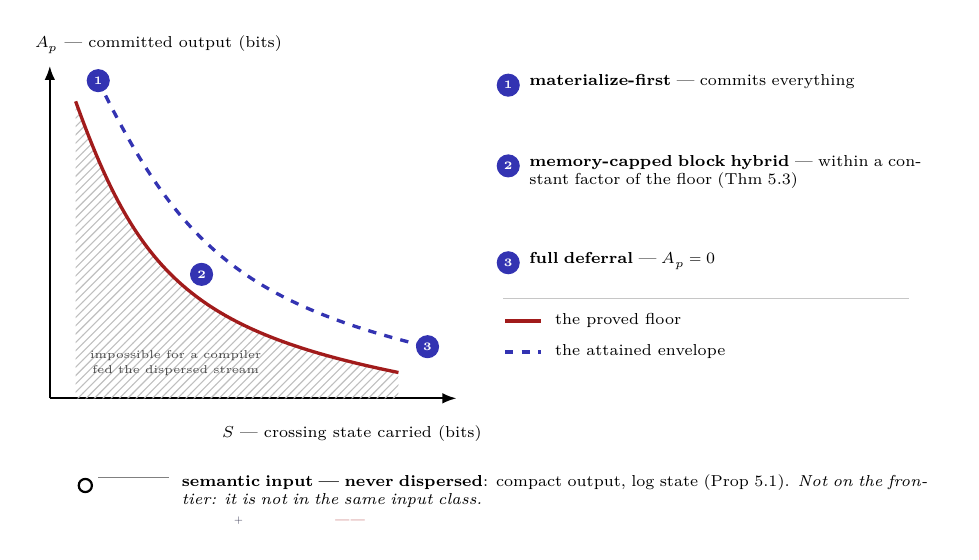
\begin{tikzpicture}[scale=0.82,transform shape,
      ar/.style={-{Latex[length=1.8mm]}},
      mk/.style={circle,draw=calblue,fill=calblue,text=white,inner sep=0pt,
                 minimum size=3.4mm,font=\tiny\bfseries},
      ky/.style={anchor=north west,align=left,font=\scriptsize,
                 text width=62mm,inner sep=0pt}]

    % ================= plot area =================
    \draw[ar,thick] (0,0) -- (6.3,0);
    \node[anchor=north west,align=left,font=\scriptsize] at (2.55,-0.30)
      {$S$ --- crossing state carried (bits)\\
       \zhtik{过切口携带的状态（比特）}};
    \draw[ar,thick] (0,0) -- (0,5.15);
    \node[anchor=south west,align=left,font=\scriptsize] at (-0.35,5.22)
      {$A_p$ --- committed output (bits)\quad\zhtik{已提交输出（比特）}};

    % impossible region
    \path[pattern=north east lines,pattern color=gray!50]
      (0.40,4.60) .. controls (1.35,1.95) and (2.20,1.05) .. (5.40,0.40)
      -- (5.40,0) -- (0.40,0) -- cycle;
    \draw[very thick,mustred]
      (0.40,4.60) .. controls (1.35,1.95) and (2.20,1.05) .. (5.40,0.40);
    \draw[very thick,dashed,calblue]
      (0.75,4.92) .. controls (1.95,2.45) and (2.95,1.50) .. (5.85,0.80);

    \node[font=\tiny,gray!55!black,align=center] at (1.95,0.46)
      {impossible for a compiler\\ fed the dispersed stream\\
       \zhtik{喂给打散流的编译器到不了这片区域}};

    % markers on the curve
    \node[mk] at (0.75,4.92) {1};
    \node[mk] at (2.35,1.92) {2};
    \node[mk] at (5.85,0.80) {3};

    % ================= key on the right =================
    \node[mk] at (7.10,4.85) {1};
    \node[ky] at (7.42,5.02)
      {\textbf{materialize-first} --- commits everything\\
       \zhtik{全部提前承诺：输出最大，状态最小}};

    \node[mk] at (7.10,3.60) {2};
    \node[ky] at (7.42,3.77)
      {\textbf{memory-capped block hybrid} --- within a constant
       factor of the floor (Thm 5.3)\\
       \zhtik{内存受限的分块混合：距地板仅一个常数因子}};

    \node[mk] at (7.10,2.10) {3};
    \node[ky] at (7.42,2.27)
      {\textbf{full deferral} --- $A_p=0$\\
       \zhtik{完全延迟：一个比特都不提交，全部扛在状态里}};

    \draw[gray!45] (7.02,1.55) -- (13.3,1.55);
    \draw[very thick,mustred]        (7.05,1.20) -- (7.60,1.20);
    \node[anchor=west,font=\scriptsize] at (7.70,1.20)
      {the proved floor \zhtik{已证明的地板}};
    \draw[very thick,dashed,calblue] (7.05,0.72) -- (7.60,0.72);
    \node[anchor=west,font=\scriptsize] at (7.70,0.72)
      {the attained envelope \zhtik{构造达到的包络}};

    % ================= the isolated semantic point =================
    \draw[thick] (0.55,-1.35) circle (2.9pt);
    \draw[thin,gray] (0.75,-1.22) -- (1.85,-1.22);
    \node[anchor=north west,align=left,font=\scriptsize,text width=118mm]
      at (1.92,-1.06)
      {\textbf{semantic input --- never dispersed}: compact output, log state
       (Prop 5.1). \emph{Not on the frontier: it is not in the same input
       class.}\\
       \zhtik{语义输入，从未被打散：紧凑输出 $+$ 对数状态。它不在前沿上，}%
       \zhtikem{是因为它根本不属于同一个输入类——这条界不是在说编译器做不好。}};
  \end{tikzpicture}
\end{frame}

% ---------------------------------------------------------------- Frame 5.6
\begin{frame}{\bl{Scope: the seven assumptions and where each breaks}%
                {Scope：七条假设，以及各自在哪里失效}}
  \zhsub{Scope：七条假设，以及各自在哪里失效}
  \footnotesize
  \begin{center}
  \begin{tabular}{@{}p{0.34\textwidth} p{0.58\textwidth}@{}}
    \toprule
    assumption & what breaks without it\\
    \midrule
    $\Fb$-independence
      & Lemma 1.4 surjectivity fails $\Rightarrow$ first step of Thm 1.7
        cannot be executed\\
    contiguity
      & commutation premise (Frame 0.4) fails $\Rightarrow$ \alert{the
        aggregate does not exist} $\Rightarrow$ the \emph{question} fails, not
        the bound\\
    coefficient freedom across rounds
      & fooling set collapses to one class (constant schedule, Frame 3.4)\\
    $Q\ge3$
      & no common suffix $v_j$ exists in Thm 4.2\\
    $\varepsilon<\sin(\pi/2Q)$
      & decoder of Lemma 1.10 fails $\Rightarrow$ Fano unusable\\
    $\delta<1/2$
      & $\Ldelta$ in $(0.2)$ loses meaning\\
    Lemma 3.5 condition $(3.2)$
      & rounds accumulate in different bases $\Rightarrow$ coordinate
        structure of Def 3.1 lost\\
    \bottomrule
  \end{tabular}
  \cn{七条假设失效时坏掉的东西各不相同。特别注意第二行：失去 contiguity 时，坏掉的是"aggregate 存在"这个前提，也就是问题本身，而不是界。}
  \end{center}
\end{frame}

% ---------------------------------------------------------------- Frame 5.7
\begin{frame}{\bl{Takeaway}{收束}}
  \zhsub{收束}
  \vfill
  \begin{center}
  \begin{minipage}{0.88\textwidth}
    \begin{block}{}
      \begin{center}\LARGE\alert{Randomize and lower late.}\end{center}
      \bigskip

      \normalsize
      The information a compiler discards before aggregating cannot be
      recovered for free --- it must be bought back \alert{in memory} or
      \alert{in magic states}, and buying it back early is strictly the more
      expensive of the two.
      \bigskip

      \begin{center}
        \textbf{Treat recoverability as a controlled variable in compilation
        and resource estimation.}
      \end{center}
      \cn{编译器在聚合之前丢掉的信息，不可能免费取回——只能用内存或magic state买回来，而且早买严格更贵。请把 recoverability 当作编译与资源估计中的一个受控变量。}
    \end{block}
  \end{minipage}
  \end{center}
  \vfill
  \note{回到 Frame 0.2 的三行。最后一句是给听众的行动建议：
        把 recoverability 当作编译与资源估计中的一个受控变量。}
\end{frame}

%%%%%%%%%%%%%%%%%%%%%%%%%%%%%%%%%%%%%%%%%%%%%%%%%%%%%%%%%%%%%%%%%%%%%%%%%%%%%%
%  PART VII  ==  Appendix / Backup   (after §5; not part of the 0-5 main line)
%%%%%%%%%%%%%%%%%%%%%%%%%%%%%%%%%%%%%%%%%%%%%%%%%%%%%%%%%%%%%%%%%%%%%%%%%%%%%%
% ------------------------------------------------ Frame 6.0 -- closing frame
\begin{frame}[plain]
  \vfill
  \begin{center}
    {\Huge\color{calblue}\textbf{Thanks for listening.}}\\[3mm]
  \end{center}
  \vfill
  \note{正文到此结束。留在这一页接受提问；后面全部是 backup，
        被问到再翻：A.1 证据分级、A.2 三个可证伪实验、A.7 可证伪性一句话。}
\end{frame}

\appendix
\AtBeginSection[]{}
% keep the theme footline, but flag every appendix page as BACKUP
\renewcommand{\footcellauthor}{\textbf{BACKUP}}

% ---------------------------------------------------------------- Frame A.1
% (first frame of the appendix, per the spec checklist)
\begin{frame}{\bl{A.1 Evidence classes (Table IV)}{A.1 证据分级（表 IV）}}
  \zhsub{A.1 证据分级（表 IV）}
  \scriptsize
  \begin{center}
  \begin{tabular}{@{}p{0.20\textwidth} p{0.34\textwidth} p{0.38\textwidth}@{}}
    \toprule
    class & contents & authorized inference\\
    \midrule
    \ding{192}\,\textbf{instrumented theorem-model implementation}
      & traced reference compilers $+$ restart verifier (592 runs)
      & \alert{directly tests the serialized commitment--cut coordinates; can
        falsify the theorems}\\
    \ding{193}\,\textbf{configured-pipeline diagnostic}
      & matched matrix, external semantic baselines, exact-semantics
        witnesses, natural workloads
      & compares observed tool behaviour; \alert{never proves a lower bound}\\
    \ding{194}\,\textbf{model-specific consequence}
      & fixed-total-error synthesis $+$ surface-code calculation
      & reports consequences under the \alert{disclosed} QRE; \alert{not a
        hardware-independent forecast}\\
    \bottomrule
  \end{tabular}
  \cn{三类证据的授权推断范围不同：只有类别 \ding{192} 能证伪定理；类别 \ding{193} 只比较工具的实际行为，永远不能证明下界；类别 \ding{194} 只在已披露的 QRE 假设下报告后果，不是硬件无关的预测。}
  \end{center}
  \note{这是所有"你的实验能证明什么"类攻击的挡箭牌。
        先讲这一帧，再讲 A.2。三个类别的授权推断范围要能背下来。}
\end{frame}

% ---------------------------------------------------------------- Frame A.2
\begin{frame}{\bl{A.2 Only three experiments can falsify the theory}%
                {A.2 只有三个实验能证伪理论}}
  \zhsub{A.2 只有三个实验能证伪理论}
  \scriptsize
  \hd{Fig 5 --- trace-derived frontier (592 runs) $\to$ tests Theorem 4.6.}
  Measures the theorem's own coordinates $A_p$, $S$, IR share; the black edge
  is the measured Pareto set, the theoretical lower envelope evaluated
  \alert{in the same serialized-bit coordinates}. All frozen points lie in the
  theorem-allowed region; no point removed as an outlier.
  \emph{Falsification: any point below the envelope kills Theorem 4.6.}
  (Echo occupies the early-commit corner; full aggregation the state-heavy
  compact-output corner; three capped hybrids interpolate --- matching the
  three constructions of Part VI.)
  \smallskip

  \hd{Fig 2 --- $\eta$ sweep $\to$ tests Proposition 6 and ``two currencies''.}
  Left: a deferred compact-output compiler pays dispersal in crossing state;
  slopes $10.3/21.1/43.3$ bytes per unit $\eta$ at $m=32/64/128$, sitting on
  the zero-error floor $\eta m(\log_23+1)/8$ bytes (ratios $0.99$--$1.05$).
  \emph{Read the floor:} $\log_23=1.585$ bits of residue $+1$ bit of
  sign/frame $=2.585$. Right: a streaming compiler pays the same dispersal in
  committed prefix (slopes $60/129/260$, larger by the public addresses) while
  its crossing state stays flat at $\le8$ bytes.
  \emph{Falsification: no tradeoff between panels, or state channel below the
  floor.}
  \smallskip

  \hd{Fig 3 --- commitment toll, preregistered $\to$ tests Theorem 4.8 $+$
  Corollary 4.9.}
  Four serializers at $m\in\{128,512,2048\}$ (two up to $m=32768$), every cell
  restart-verified: matches $\log_2\binom mk/k$ within $0.17$ bits worst case,
  $0.02$ typically; \alert{flat in $m$} at fixed $\eta$
  ($2.11/1.99/1.97$ at $\eta=\frac12$ across a $16\times$ range);
  \alert{exactly zero at $\eta=1$}; \alert{exactly zero at every $\eta$ in the
  control} (prefix omits the mask, recovers it from the suffix).
  \emph{Falsification: toll growing with $m$, or nonzero in the control, or
  nonzero at $\eta=1$.}
  \cn{三个实验，三条证伪条件：Fig 5 只要有一点落在包络之下，Theorem 4.6 就死；Fig 2 只要两个面板之间没有 tradeoff、或状态通道低于地板；Fig 3 只要 toll 随 $m$ 增长、或对照组非零、或 $\eta=1$ 时非零。}
  \note{三个可证伪实验的名字、坐标和证伪条件都要能脱口而出。
        Fig 3 的四条断言正好就是推论 4.9 的四条。}
\end{frame}

% -------------------------------------------------------------- Frame A.2b
\begin{frame}{\bl{A.2 (cont.) Fig 3: what the control experiment shows}%
                {A.2（续）Fig 3：对照实验说明了什么}}
  \zhsub{A.2（续）Fig 3：对照实验说明了什么}
  \small
  \begin{callout}
    The control (prefix omits the mask, recovers it from the suffix) is
    \alert{exactly zero at every $\eta$}. This shows that
    \alert{irreversibility of commitment, not addressing, is what buys the
    asymmetry.}
    \cn{对照组（前缀不写 mask，由后缀恢复）在每个 $\eta$ 上都恰好为零。这说明买到不对称的是承诺的不可逆性，不是寻址。}
  \end{callout}
  \smallskip

  \footnotesize
  Right panel: under an identity-optimal serializer the ratio is $1.00$ at
  $\eta=1$ and $\le2.64$ throughout --- the $6{:}1$ of Fig 2 is \alert{codec
  slack}, and only the slack grows with address width ($5.4{:}1$ at $m=128$ to
  $10.8{:}1$ at $m=32768$).
  \smallskip

  \alert{The preregistration recorded ``there is no address-width law here''
  as a prediction against the natural reading of Fig 2, and it is reported as
  such.}
  \note{这一帧的作用是防守"你的 6:1 是不是地址宽度效应"。
        答案：那是编解码器的余量，不是定律；而且我们预先登记过这个预测。}
\end{frame}

% ---------------------------------------------------------------- Frame A.3
\begin{frame}{\bl{A.3 Diagnostics (class \ding{193}): what they do and do not
                  show}%
                {A.3 诊断实验（类别 \ding{193}）：能说明与不能说明什么}}
  \zhsub{A.3 诊断实验（类别 \ding{193}）：能说明与不能说明什么}
  \scriptsize
  \begin{itemize}
    \item \hd{Fig 8 $+$ Table VII --- mechanism ablation.} With Fourier-layer
          IR disabled, the compiler completes at 4k/10k/20k but materializes
          outputs of the same order as \texttt{qiskit opt3}, and exceeds the
          600\,s budget at 50k/100k; enabled, it returns the same 42-gate
          circuit at every scale. \alert{The constant form is caused by
          semantic lifting $+$ coefficient aggregation, not by a lucky pass
          ordering.} (This is the only experiment answering that objection.)
    \item \hd{Fig 6/7 $+$ Tables XIII/XIV --- exact-semantics witnesses}
          (Corollary 1, $\varepsilon=0$, fixed width). Semantic UCC constant
          (42 rational / 27 irrational). \alert{Rebased TKET PauliSimp
          recovers a small validated form at all five scales (52--73 /
          35--38)} --- the classification's \emph{positive} prediction.
          staq / \texttt{qiskit opt3} / GuidedPauliSimp grow linearly.
          \alert{None of these is an impossibility result.}
    \item \hd{Fig 4 --- matched matrix (1080 cells).} Same target, basis,
          budget, seed; \alert{only the representation varies.}
          (a) certified completion probability, (b) serialized output size
          among completed cells only. masked-share $\times$ Qiskit L3
          completes at $0.38$ (\texttt{predicate\_error}), \alert{retained as
          a status observation, never scored as a numerical loss.}
    \item \hd{Tables V/VI.} Table V is explicitly \alert{not} an instance of
          the masked-share lower bound (balanced encoding tokens contain
          $x_j/r$, hence leak the aggregate). Table VI tests Prop 13: output
          constant in $r$, $O(m_{\mathrm{CP}})=O(n(n-1)/2)$ across widths.
    \item \hd{Certificate audit.} 56 adversarial mutations (angle, sign,
          support bit, qubit permutation, Clifford frame, deletion,
          duplication) with \alert{0 false accepts}; 12 dense/symbolic
          cross-checks at $n\le6$ with no disagreement. This is what makes
          ``only \texttt{completed\_valid} enters quality means'' meaningful.
  \end{itemize}
  \cn{这一整页都是类别 \ding{193}：只比较工具的实际行为，不构成任何不可能性结果。Fig 8 是唯一回答"是不是碰巧的 pass 顺序"的实验；Fig 6/7 里外部 TKET 恢复出小形式，是分类的正面预言，要主动承认。}
  \note{类别②的实验一律不用来支持下界。
        Fig 8 是唯一回答"是不是碰巧的 pass 顺序"的实验；
        Fig 6/7 里 TKET 恢复出小形式，是分类的正面预言，要主动承认。}
\end{frame}

% ---------------------------------------------------------------- Frame A.4
\begin{frame}{\bl{A.4 The E7 preregistered TKET scan: report, do not repair}%
                {A.4 E7 预登记 TKET 扫描：只报告，不修补}}
  \zhsub{A.4 E7 预登记 TKET 扫描：只报告，不修补}
  \small
  $m\in\{8,16,32,64,128\}$, three seeds, byte-identical pass sequence. TKET
  achieved compact output in \alert{every} cell (508 dispersed rotations
  $\to$ 127 non-Clifford $R_z$ at $m=128$); its pass-phase memory and
  serialized IR grew with log--log slope $\approx1.7$ in $m$, while the
  instrumented semantic-input control stayed flat ($196\to199$ bytes over a
  $16\times$ range).
  \smallskip

  \begin{callout}
    \alert{The preregistered point prediction of exactly linear growth was
    rejected under its own frozen decision rule, and is reported as rejected.}
    \cn{预登记的"严格线性增长"点预测，在它自己的冻结判定规则下被否决，并按被否决如实报告。}
  \end{callout}
  \vspace{-1mm}

  \scriptsize Two scope limits, stated explicitly:
  \begin{enumerate}\scriptsize
    \item What is measured at a third-party API boundary is a pass-phase
          memory and serialized-IR snapshot --- \alert{class \ding{193}; not
          promoted to a measurement of $\Bcut$, and not commensurable with the
          $S$ of the frontier.} The scan tests only the qualitative dichotomy
          (dispersed input forces growth in $m$; semantic input does not) ---
          neither the constant nor the exponent.
    \item Superlinear growth means \alert{the floor is not the binding
          constraint on this tool}: the bound establishes the floor, the
          observed cost exceeds it, and the excess is implementation structure
          (the pairwise commutation structure of a Pauli graph is itself
          superlinear in the number of terms). \alert{No claim that our
          implementation outperforms these tools.}
  \end{enumerate}
  \note{预登记失败要主动报告，不要修补。
        并且要说清楚：超线性意味着下界不是这个工具的约束瓶颈，
        多出来的部分是实现结构，不是我们的功劳。}
\end{frame}

% ---------------------------------------------------------------- Frame A.5
\begin{frame}{\bl{A.5 Consequences (class \ding{194}): the QRE campaign}%
                {A.5 后果（类别 \ding{194}）：QRE campaign}}
  \zhsub{A.5 后果（类别 \ding{194}）：QRE campaign}
  \small
  Table VIII $+$ Fig 9 $+$ Fig 13, \alert{288 rows}. One fixed
  $\varepsilon_{\mathrm{total}}$ split additively: $0.10$ algorithmic, $0.45$
  rotation synthesis, $0.45$ logical failure. \alert{Every angle actually
  synthesized} by a frozen deterministic GMP build of staq
  \texttt{grid\_synth} (670 angle--precision pairs; reported error never
  exceeds the allocated radius).
  \smallskip

  Across all 96 matched target/error/allocation/QEC/factory settings:
  materialize-first uses \alert{385--1753$\times$} the logical $T$ states and
  \alert{538--5573$\times$} the spacetime volume of semantic-first.
  \alert{No reversal in the scanned grid.}
  \smallskip

  \begin{callout}[\bl{Two things to volunteer}{两件要主动说的事}]
    \footnotesize
    \begin{enumerate}
      \item This is \alert{not} a claim that our implementation dominates
            other semantic tools --- external \textbf{TKET PauliSimp uses
            0.443--0.536$\times$ our $T$ states} on this witness, i.e.\ it is
            better, and crediting that recovery is part of the comparison.
      \item Absolute physical numbers still depend on routing, correlated
            errors, factory layout, feed-forward and code-distance
            assumptions. \alert{Not a hardware-independent forecast.}
    \end{enumerate}
    \cn{两件要主动交代：外部 TKET PauliSimp 在这个 witness 上只用我们 $0.443$–$0.536$ 倍的 $T$ 态，即它更好；绝对物理数字仍依赖 routing、相关误差、factory 布局等一整套已披露假设。}
  \end{callout}
  \note{$10^2$–$10^3$ 倍的差距很吓人，所以更要主动交出两条限制：
        （1）外部 TKET 在这个 witness 上比我们好，要给它记功；
        （2）绝对物理数字依赖一整套披露过的架构假设。}
\end{frame}

% ---------------------------------------------------------------- Frame A.6
\begin{frame}{\bl{A.6 Honest nulls and anti-regression}%
                {A.6 诚实的零结果与防回归}}
  \zhsub{A.6 诚实的零结果与防回归}
  \small
  \begin{itemize}
    \item \hd{Fig 10 / Table IX --- real instances.} Parity with
          \texttt{qiskit opt3}; $\approx65\%/73\%/78\%$ gate reduction against
          the upstream UCC v0.4.12 pre-semantic default. \alert{The paper
          explicitly states this is an anti-regression check, not evidence of
          semantic recovery.}
    \item \hd{Fig 11/12 $+$ Table X --- W8 six-factor ablation (21{,}060
          cells).} Preset recognizer largest main effect (mean reduction
          $364.9$, bootstrap CI $[349.8,380.5]$); \alert{selector,
          cache/reuse and projected-block selection have exactly zero isolated
          effect.} Both negative controls show zero all-on-minus-all-off
          differences in gates, depth, CX, logical $T$ and spacetime.
          \alert{Five structured families meet the predeclared
          all-size/all-seed criterion; QFT arithmetic and phase-polynomial
          blocks do not and are retained in the table.}
  \cn{零结果照登不删：Fig 10 只是防回归检查，不是语义恢复的证据；W8 消融里三个因子的孤立效应恰好为零，两个族没有达到预先声明的标准，都保留在表里。}
  \end{itemize}
  \note{零结果要保留在表里，不要删。
        "三个因子的孤立效应恰好为零"和"两个族没有达标"都是主动交代的项。}
\end{frame}

% ---------------------------------------------------------------- Frame A.7
\begin{frame}{\bl{A.7 The falsifiability one-liner}{A.7 可证伪性一句话}}
  \zhsub{A.7 可证伪性一句话}
  \vfill
  \begin{center}
  \begin{minipage}{0.90\textwidth}
    \begin{mustanswer}[\bl{If you remember one defensive sentence}%
                         {只记一句防守用的话}]
      \normalsize
      \alert{Only three experiments can falsify my theorems:} Fig 5 (the
      frontier envelope), Fig 2 (the two channels and the floor), Fig 3 (the
      four predictions of the toll).
      \bigskip

      Everything else is either a configured-pipeline diagnostic or a
      consequence under a disclosed model --- \alert{I use none of it to
      support any lower bound.}
      \bigskip

      \alert{Two third-party preregistrations failed; I report them rather
      than repair them.}
      \cn{只有三个实验能证伪我的定理：Fig 5、Fig 2、Fig 3。其余要么是 configured-pipeline 诊断，要么是已披露模型下的后果——我不用它们支持任何下界。两个第三方预登记失败了，我如实报告而不修补。}
    \end{mustanswer}
  \end{minipage}
  \end{center}
  \vfill
  \note{这句话把"你的实验能证明什么"这个开放式攻击，
        压缩成一个你已经先答完的封闭问题。全场最强装备，留在最后。}
\end{frame}

% ---------------------------------------------------------------- Frame A.8
\begin{frame}{\bl{A.8 Reproducibility (only if asked)}%
                {A.8 可复现性（被问到才讲）}}
  \zhsub{A.8 可复现性（被问到才讲）}
  \footnotesize
  \begin{itemize}
    \item Canonical registry \texttt{data/manifest.yaml}; normalized Parquet
          index with \alert{24{,}748 unique records}, retaining \alert{48
          predicate-error rows outside quality means}.
    \item Primary key: \texttt{experiment\_id, instance\_id,
          representation\_id, method\_id, seed, backend\_hash, tool\_version,
          artifact\_commit, config\_hash}.
    \item Every printed number traced to a unique source row via
          \texttt{data/provenance\_map.yaml}, tested by
          \texttt{tests/test\_paper\_number\_provenance.py}.
    \item One-command entry point
          \texttt{reproducibility/run\_submission.sh}: reruns audits,
          regenerates all tables/figures, executes the test suite, builds the
          manuscript, rejects unresolved references.
    \item Clean-room runner: independent temporary directory $+$ fresh
          environment on locked packages; reconstructs 9 headline-theorem
          tests, one certified QAOA/Ising instance through both paths, 17
          deterministic synthesis pairs. \alert{This is working-directory
          isolation, not host-binary independence.}
  \cn{每一个印出来的数字都能经 \texttt{provenance\_map.yaml} 追到唯一源行，并有测试守着。最后一条要主动说：clean-room 是工作目录隔离，不是宿主二进制独立。}
  \end{itemize}
  \note{最后一条要主动说：clean-room 是工作目录隔离，不是宿主二进制独立。
        不要让别人替你指出来。}
\end{frame}

\end{document}
